\chapter{Placement de contre-mesures logicielles}
\label{chpt:placement}
    
    Ce chapitre se concentre sur les contre-mesures logicielles et présente une méthodologie de placement de contre-mesures en fautes multiples combinant une analyse en isolation des schémas de protection et différents algorithmes de placement automatique.      

    La section \ref{sec:soa-countermeasures} présente les problématiques de l'analyse de contre-mesures et comment les méthodologies proposées dans ce chapitre peuvent être utilisées pour y répondre. 
    Cette section s'intéresse aussi à quelques contre-mesures logicielles et leurs caractéristiques, ainsi que les approches existantes dans le domaine de l'évaluation et la comparaison de programmes protégés.
    La section \ref{sec:ch6-defs} traite des différentes contre-mesures automatiques proposées dans Lazart et introduit certaines propriétés nécessaires aux algorithmes de placement.
    La section \ref{sec:placement} présente les algorithmes de placement automatique de contre-mesures et discute des garanties qu'ils apportent en fonction des contre-mesures considérées.
    La section \ref{sec:placement-exps} discute des expérimentations qui ont été réalisées pour ces différents algorithmes.
    La section \ref{sec:model-protectability} s'intéresse à la notion de "protégeabilité" des modèles de faute et propose une classification correspondante.
    Finalement, la section \ref{sec:placement-fw} discute des perspectives de ces travaux. 
    
    \section*{Table des Matières}
    \localtableofcontents
    
    \section{Chaîne de développement logiciel et analyse de contre-mesures}
    \label{sec:soa-countermeasures}
    
        Les chapitres précédents ont introduit les notions de contre-mesures et d'analyse de contre-mesures (section \ref{sec:fi-protections}).
        La suite de ce manuscrit s'intéresse plus particulièrement à la protection de programmes au niveau logiciel.
        
        \begin{defi}
            \label{def:countermeasure}
            Une contre-mesure est une transformation d'un système (programme, algorithme, composant) qui préserve son comportement observable en l'absence d'attaque et vise à augmenter la sécurité en présence d'attaques.
        \end{defi}
                
        L'\textit{analyse de contre-mesure} a déjà été abordée dans les chapitres précédents, et plusieurs problématiques ont été énoncées :
        \begin{itemize}
            \item \textit{le placement :} comment sélectionner les contre-mesures et leurs positions dans un programme.
            \item \textit{la comparaison :} comment comparer et évaluer des contre-mesures et des programmes protégés.
            \item \textit{l'optimisation :} comment déterminer si les protections ajoutées sont effectivement utiles ou si certaines peuvent être retirées.
        \end{itemize}
        
        Ces différentes problématiques sont liées les unes aux autres. Entre autres:
        \begin{itemize}
            \item la capacité de comparer les contre-mesures, pour un modèle d'attaquant donné, permet d'aider au placement des contre-mesures,
            \item l'optimisation de programme peut être utilisée pour placer des contre-mesures en les appliquant systématiquement sur le programme et en calculant a posteriori une version réduite de celui-ci.
        \end{itemize}
        
        La section \ref{sec:cm-soa} s'intéresse à quelques contre-mesures logicielles de la littérature et discute de leurs caractéristiques.
        La section \ref{sec:cm-analysis} présente une revue des techniques d'analyse de contre-mesures proposées dans la littérature.
        Finalement, la section \ref{sec:cm-concl} propose une synthèse de cette section.

        \subsection{Contre-mesures}
        \label{sec:cm-soa}
        
            La section \ref{sec:fi-protections} a présenté les caractéristiques des contre-mesures en fonction du niveau de représentation considéré.
            Cette section se concentre sur les contre-mesures logicielles (ce qui inclut les transformations au niveau assembleur/binaire) et vise à présenter différentes caractéristiques, qui permettront notamment de classifier les contre-mesures pour s'intéresser aux garanties apportées par les algorithmes de placement. 
            Les contre-mesures visant les attaques par canaux-auxiliaires ou visant spécifiquement la protection d'implémentations cryptographiques ne sont pas considérées ici.
            
            La table \ref{tbl:cm-comparison} présente différentes contre-mesures logicielles proposées dans la littérature. 
            La colonne "Nom" indique la contre-mesure en question et "Date" l'année de la publication. Les contre-mesures préfixée par "LZ" correspondent aux contre-mesures automatiques implémentées par Lazart: multiplication de tests ("LZ TM"), multiplication de loads ("LZ LM") et une implémentation de SecSwift \cite{Ferriere/LLVM19} ("LZ SSCF"). 
            
            Les colonnes suivantes correspondent aux différentes classes de caractéristiques qui sont présentées dans cette section: "Modèle" (caractéristiques relatives au modèle de faute et au niveau de représentation), "Méthode" (caractéristiques liées à l'implémentation et le fonctionnement de la contre-mesure) et "Application" (caractéristiques concernant l'application de la contre-mesure sur un programme).
            
            \begin{table}[h]
                {\footnotesize
                \begin{center}
                \setlength\tabcolsep{3pt}
                \begin{tabular}{lll|lll|ll|llll}
                \multicolumn{3}{l|}{Général} & \multicolumn{3}{l|}{Modèle} & \multicolumn{2}{l|}{Méthode} & \multicolumn{4}{l}{Application} \\
                \hline
                Nom & Famille & Date & Dom. & Modèle & MF & Etat & Tech. & Niveau & Granu. & Auto. & Syst. \\
                \hline
                \hline
                Booléen durcis & Data & - & FA & Data & 1 & non & L & - & V & oui & F \\
                \begin{tabular}[c]{@{}l@{}}CFCSS\\ \cite{Oh/TR02}\end{tabular} & Both & 2002 & FT & bit-flip & 1 & oui & D / I & Compil. & B & oui & \cellcolor[HTML]{FFFFFF}P \\
                \cite{nicolescu2004software} & Both & 2003 & FT & bit-flip & 1 & oui & D / I & Compil. & I/B & oui & P \\
                \begin{tabular}[c]{@{}l@{}}Swift\\ \cite{Reis/ISCCO05}\end{tabular} & Both & 2005 & FT & CF & 1 & oui & D / I & LLVM & G & oui & P \\
                Lalande & CFI & 2014 & FA & Saut & 1 & oui & D / I & C & SL & oui & F \\
                \cite{Moro/Phd14} & Both & 2014 & FA & CF/Data & 1 & oui & D / I & Binaire & I & oui & P \\
                \begin{tabular}[c]{@{}l@{}}SecSwift\\ \cite{Ferriere/LLVM19}\end{tabular} & CFI & 2019 & FA & CF & X & oui & D / I & LLVM & F/B & oui & F \\
                LZ TM & CFI & 2019 & FA & TI & X & non & D & LLVM & IP & oui & - \\
                LZ LM & Data & 2022 & FA & DL & X & non & D & LLVM & IP & oui & - \\
                LZ SSCF & CFI & 2020 & FA & CF & X & oui & D / I & LLVM & IP & oui & -
                \end{tabular}
                \end{center} 
                }
                \caption{Comparaison de quelques contre-mesures logicielles \label{tbl:cm-comparison}}
            \end{table}
            
            Deux grandes \textit{familles} de contre-mesures se dégagent au niveau logiciel (colonne "Famille"), en fonction de si celles-ci visent la protection du flot de contrôle (CFI) ou du flot de données (Data). Certaines contre-mesures visent les deux à la fois \cite{Reis/ISCCO05}.
            La colonne "Modèle" indique le modèle de faute visé par la contre-mesure et la colonne "MF" précise si la contre-mesure vise les fautes multiples ("X") ou la faute unique ("1").
            La colonne "Domaine" indique si la contre-mesure est issue du domaine des attaques en fautes ("FA") ou des fautes accidentelles ("FT").
            
            La colonne "État" indique si la contre-mesure propage un \textit{état interne} (comme un compteur \cite{heydemann2019formally} ou des variables \cite{Reis/ISCCO05, Ferriere/LLVM19}) ou si chaque application n'utilise que des états du programme initial (comme la duplication de test).
            La colonne "Tech." indique quelles \textit{techniques} sont utilisées pour la contre-mesure, à savoir :
                \begin{itemize}
                    \item \textit{détection (D) :} l'état du programme est vérifié à certains points de contrôle et une réponse est déclenchée (arrêt du programme, arrêt du système ou signalement de l'erreur par exemple). 
                    \item \textit{infection (I)} : les sorties du programmes sont rendues inutilisables ou invalides en cas de faute.
                    \item \textit{dilution (L)} : l'attaque est rendue plus difficile à réaliser, sans la bloquer complètement.
                \end{itemize}
            
            Pour la catégorie "Application", le \textit{niveau de représentation} (colonne "Niveau"), précise à quel niveau la contre-mesure est appliquée (langage source, représentation intermédiaire ou compilation). 
            La colonne "Granu." correspond à la \textit{granularité} de l'application de la contre-mesure sur le programme, c'est-à-dire quels types de structures peuvent être protégées indépendamment. Il peut s'agir d'une granularité globale ("G"), de l'ordre d'une fonction ("F") ou du bloc de base ("B"), de l'ordre du point d'injection ("IP"), des instructions ("I") ou encore au niveau de structures logicielles ("SL") telles que les boucles ou les conditions.
            La colonne "Automatisation" indique si la contre-mesure est destinée à être appliquée manuellement ou automatiquement (par exemple dans un compilateur).
            La colonne "Syst." indique si l'application automatique est appliquée sur l'ensemble du programme \cite{lalande} ("F") ou si les auteurs proposent une méthode pour réduire cette application en fonction de certains critères ou analyses \cite{Reis/ISCCO05} ("P"). 
            
            La \textit{performance} (c'est-à-dire le surcoût de temps d'exécution, de consommation mémoire ou de taille de code) est aussi un paramètre capital pour le choix des contre-mesures à appliquer. Cette caractéristique n'est pas présentée dans la table ci-dessus.

        \subsection{Évaluation de contre-mesures}
        \label{sec:cm-analysis}
    
            L'évaluation de contre-mesures vise à répondre à deux questions principales :
            \begin{itemize}
                \item Déterminer quelle contre-mesure est la plus efficace pour un modèle de faute donné parmi un ensemble de contre-mesures.
                \item Vérifier l'efficacité des protections insérées dans un programme protégé.
            \end{itemize}
        
            Deux grandes classes d'approches se dégagent de la littérature: l'\textit{évaluation expérimentale} à l'aide d'outils d'analyse de robustesse et l'utilisation des \textit{méthodes formelles}.
    
            \subsubsection{Évaluation expérimentale de la robustesse}
            
                Une première approche consiste à comparer les résultats d'analyse de robustesse d'un programme protégé par différentes contre-mesures. En fonction de la méthode d'évaluation de la robustesse utilisée, les métriques obtenues peuvent être très variées.
                Dans un article de 2013, Thie{\ss}ing et al \cite{theissing2013comprehensive} proposent une comparaison de différents schémas de protection au niveau assembleur. Ils évaluent un ensemble de 19 contre-mesures combinant protection du flot de contrôle et des données en comparant leur surcoût en terme de mémoire et de performance, ainsi que la couverture de détection pour des fautes injectées dans les programmes d'exemples.
                Les différentes versions protégées sont comparées à l'aide d'un simulateur sur une architecture ARM en effectuant des fautes bit-flip sur les instructions et la mémoire.
                Dans \cite{Moro/HOST14}, Moro et al. proposent aussi une comparaison expérimentale de deux contremesures contre le saut d'instruction et le remplacement d'instructions au niveau binaire. 
                Cette évaluation est réalisée à l'aide d'un simulateur.
                Dans \cite{Dureuil/PPLCC16}, les auteurs présentent la collection \gls{fissc}, dont les exemples \textit{verify\_pin} et \gls{rsa} présentés précédemment sont issus.
                Les versions protégées de chaque programmes sont évaluées en inversion de test avec Lazart \cite{Potet/ICST14} au niveau \gls{llvm} ainsi qu'avec le simulateur Celtic \cite{Werner/Phd22} au niveau binaire, qui utilise un modèle de mutation de données sur les instructions.
                
                Une problématique majeure réside dans le fait que l'ajout de contre-mesures logicielles implique une augmentation 
                de la surface d'attaque du programme, les portions ajoutées pouvant elles aussi être attaquées.
                Ce \textit{paradoxe de dilution} \cite{Dureuil/Phd16}, implique qu'il est difficile de comparer les métriques sorties par les outils pour différents programmes protégés. 
                
                De plus, ces approches visent généralement la faute unique. Comparer des programmes en fautes multiples est plus coûteux en termes de temps d'analyse.
                
            \subsubsection{Méthodes formelles}
                
                Des solutions basées sur les méthodes formelles ont été proposées pour l'analyse de programmes protégés. Cette section propose quelques exemples de solutions s'appuyant sur les méthodes formelles.
                
                \textit{SymPFLIED} \cite{Pattabiraman/DSN08} (déjà abordé dans la section \ref{sec:soa-tools}) permet à l'utilisateur de spécifier un ensemble de détecteurs (de tests) sur le programme. Ceux-ci sont composés de morceaux de code écrits dans le programme à analyser à l'aide de l'instruction spécifique \texttt{assert(p)} et d'éventuelles variables fantômes nécessaires pour vérifier un prédicat $p$, qui est quant à lui spécifié en tant qu'expression dans Maude.
                Dans \cite{Pattabiraman/TC12}, un détecteur est un morceau de code externe vérifiant une propriété à l'aide d'une instruction \texttt{check}. Le détecteur est considéré comme non fautable.
                
                Dans \cite{lalande, heydemann2019formally}, les auteurs proposent une vérification formelle d'une contre-mesure, basée sur le model checking. 
                Ils parviennent ainsi à prouver que la contre-mesure proposée protège effectivement contre le modèle de faute de saut d'instructions niveau C. 
                De la même manière, Goubet et al \cite{Goubet/CARDIS15} parviennent à vérifier l'efficacité d'une contre-mesure contre le remplacement d'instructions au niveau binaire.
                Cette approche garantit qu'aucune attaque n'est possible avec le modèle de faute considéré, contrairement à des approches basées sur le test qui considèrent des entrées fixées.
                
                Martin et al. \cite{martin2022verifying} ont proposé une méthode d'analyse dans laquelle des oracles sont ajoutés manuellement pour vérifier que les contre-mesures protègent effectivement le programme contre le modèle de l'inversion de test. 
                Les inversions de tests sont représentées par un appel à une fonction \textit{mutated()} qui produit ou non une faute qui sera ajoutée à la condition par disjonction. Cette fonction vérifie que la limite de faute fournie par l'utilisateur n'est pas atteinte et retourne dans ce cas une valeur non contrainte.
                Des annotations (\gls{acsl}) sont appliquées automatiquement, vérifiant qu'aucune attaque ne peut atteindre la fin du programme sans qu'une contre-mesure ne soit déclenchée. Les annotations sont ensuite vérifiées à l'aide du plugin \gls{wp} de Frama-C.
                Les auteurs parviennent notamment à détecter une erreur dans une des contre-mesures du projet Wookey, qui avait été découverte précédemment dans \cite{inter_cesti}.
                    
        \subsection{Synthèse}
        \label{sec:cm-concl}
            
            Différentes approches ont été proposées en ce qui concerne l'analyse et l'évaluation de contre-mesures. 
            La section \ref{sec:cm-soa} a montré quelques propriétés sur les contre-mesures logicielles proposées dans la littérature.
            Néanmoins les solutions de protection sont très diverses et leur comparaison n'est pas toujours facile, sans compter le \textit{paradoxe de dilution} énoncé précédemment qui rend difficile la comparaison des métriques de robustesse, une contre-mesure pouvant ajouter de la surface d'attaque.
            
            L'approche empirique par essai / erreur est fréquemment utilisée afin de mettre en place des protections dans un programme. Cette approche ne résiste cependant pas au passage à l'échelle dans le cadre de fautes multiples.
            En effet, les contre-mesures pouvant être attaquées, l'explosion combinatoire des chemins d'attaque rend difficile l'approche empirique dans ce contexte.
            De plus, les contre-mesures et les méthodes d'analyse sont très souvent évaluées vis-à-vis d'un modèle de faute particulier, rendant le rejeu de la méthodologie difficile dans un contexte différent.
            
            La suite de ce chapitre s'intéresse à différentes stratégies de placement de contre-mesures, guidées par une recherche préalable des chemins d'attaques réussies avec Lazart.
            Ces algorithmes de placement peuvent être utilisés au sein d'outils de placement automatique de contre-mesures ou servir d'aide au développeur pour un placement manuel des contre-mesures.
        
    \section{Définitions et notions pour le placement de contre-mesures}
    \label{sec:ch6-defs}
    
        Cette section s'intéresse à quelques contre-mesures automatiques proposées dans Lazart, présente leurs schémas de protection, et définit certaines notions qui seront nécessaires pour la définition des algorithmes de placement.
        
        La section \ref{cm-local-pond} présente les notions de localité et de pondération. 
        La section \ref{sec:cm-perfection} définit la notion d'adéquation d'une contre-mesure par rapport à un modèle de faute. 
        La section \ref{sec:cm-complete} définit la notion de complétude de contre-mesures, elle aussi définie par rapport à un modèle de faute.
        Enfin, la section \ref{sec:cm-synthesis} propose une synthèse de cette section.
            
        \subsection{Localité et pondération}
        \label{cm-local-pond}
        
            Les notions de \textit{localité} et de \textit{pondération} seront illustrées respectivement par la duplication de tests (\gls{TD}) et la duplication de loads (\gls{LD}), qui sont des contres-mesures locales, et la multiplication de tests (\gls{TM}) et la multiplication de loads (\gls{LM}) qui sont des contre-mesures locales pondérées.
            Ces contre-mesures ont une granularité de l'ordre du point d'injection et on s'intéressera à leur robustesse vis-à-vis des modèles de faute \gls{TI} et \gls{DL}.
            
            \subsubsection{Contre-mesures locales au point d'injection}
            \label{sec:cm-local}
            
                La \textit{duplication de test} (\gls{TD}) est un exemple de \gls{CL} relativement au modèle d'inversion de test. La figure \ref{fig:td-scheme} présente le schéma de transformation pour la protection d'un branchement conditionnel avec cette contre-mesure dans Lazart. 
                Le \textit{schéma de protection} correspond à la règle de transformation du programme lors de l'application de la contre-mesure sur ce point d'injection. 
                Les blocs en gris correspondent au programme original et les blocs en bleu aux blocs ajoutés par la contre-mesure. Les points d'injection (pour le modèle \gls{TI}) sont indiqués en rouge, à côté de l'instruction correspondante (\texttt{br}).
                Le branchement conditionnel est dupliqué pour chaque branche (\texttt{true} et \texttt{false}) et le programme est arrêté (appel à \texttt{detect}) si le résultat n'est pas celui attendu.
                La condition (\texttt{\%cond}) n'est évaluée qu'une seule fois et est réutilisée dans les tests redondants.
                
                \begin{figure}[!tp]\centering
                    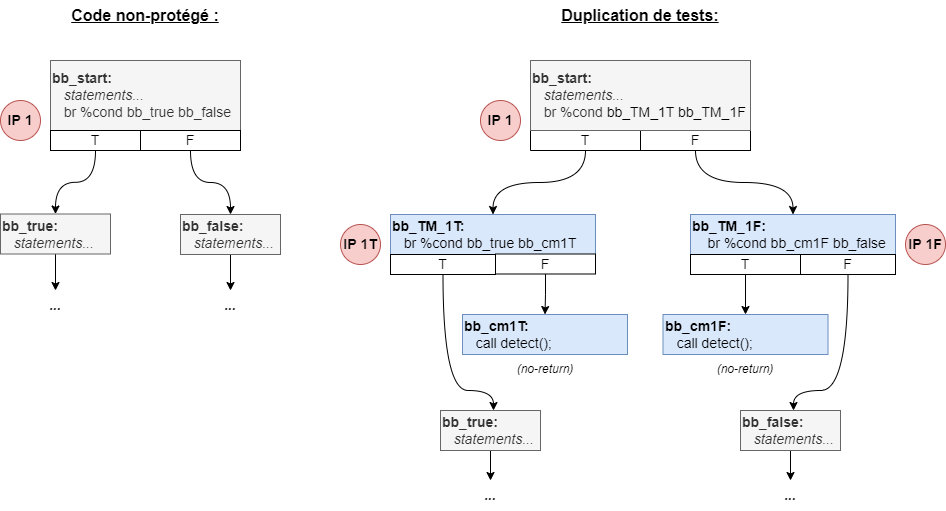
\includegraphics[scale=0.4]{ch5-placement/img/cm-mul-test-large-simple.drawio.png}
                    \caption{Schéma de protection de la duplication de test}
                    \label{fig:td-scheme}
                \end{figure}
                
                \begin{defi}
                    \label{def:cm-application}
                    Soit $P$ un programme et $C$ une contre-mesure, on note $C(P)$ l'application de $C$ sur $P$.
                \end{defi}
                \begin{defi}
                    \label{def:cm-application-local}
                    Soit $C$ une contre-mesure à granularité d'un point d'injection, on note $C(P, IP)$ l'application de $C$ localement sur le point d'injection $IP$.
                \end{defi}
                
                \begin{defi}
                    \label{def:cm-independance}
                    On dit que deux contre-mesures $C_1$ et $C_2$ sont indépendantes (noté $\perp$) ssi, pour tout programme $P$, leur ordre d'application n'a pas d'incidence\footnote{En d'autres termes, les programmes obtenus sont syntaxiquement équivalents quel que soit l'ordre d'application des contre-mesures.} sur le programme protégé obtenu :
                    $C_1 \perp C_2 \leftrightarrow C_2(C_1(P)) = C_1(C_2(P))$.
                \end{defi}
                
                \begin{defi}
                    \label{def:cm-local}
                    Pour un modèle de faute $m$, une contre-mesure $C$ est dite \textit{locale}, ssi, pour tout programme $P$, toutes les applications de C pour chaque point d'injection sont indépendantes: $\forall IP_a, IP_b \in IP(P), C(P, IP_a) \perp C(P, IP_b)$.
                \end{defi}
                
                \gls{TD} est une contre-mesure locale (définition \ref{def:cm-local}), puisqu'elle s'applique sur les points d'injection d'inversion de test (granularité \gls{ip}) et chaque application est indépendante (définition \ref{def:cm-independance}).
                Cette notion de \textit{localité} est importante pour le placement de contre-mesures, puisque dans le cas de contre-mesures locales, il est possible de représenter l'application de la contre-mesure comme un ensemble non ordonné de points d'injection.
                
            \subsubsection{Contre-mesures locales pondérées}
            \label{sec:cm-ponderated}
    
                La multiplication de tests est un exemple de contre-mesure locale pouvant être appliquée avec un niveau de pondération différent pour chaque point d'injection.
                On parle alors de \gls{CLP}, et on appelle \textit{profondeur} le coefficient d'application d'une contre-mesure pour un point d'injection donné (définition \ref{def:cm-ponderated}).
                
                \begin{figure}[p]\centering
                    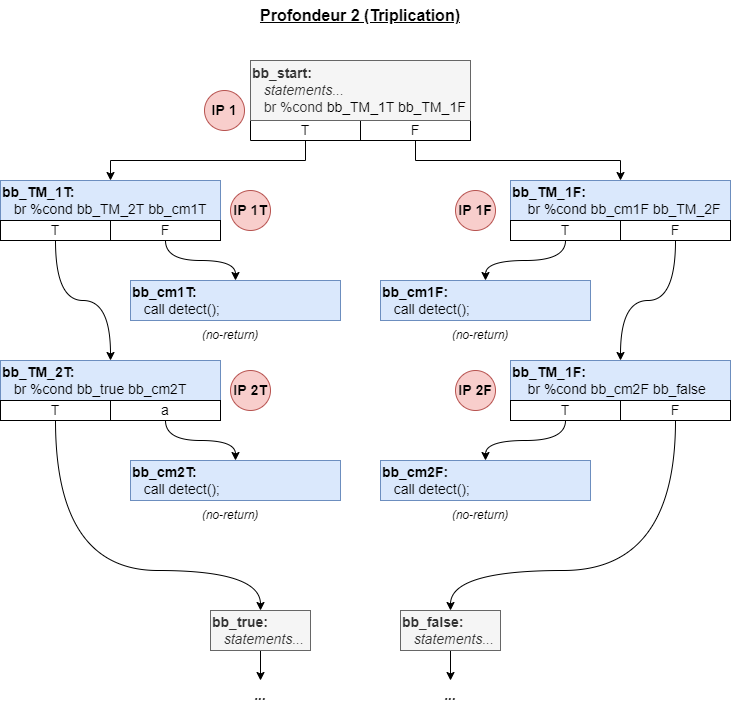
\includegraphics[scale=0.45]{ch5-placement/img/cm-mul-tripl.png}
                    \caption{Schéma de protection de la triplication de test}
                    \label{fig:tt-scheme}
                \end{figure}
            
                \begin{figure}[p]\centering
                    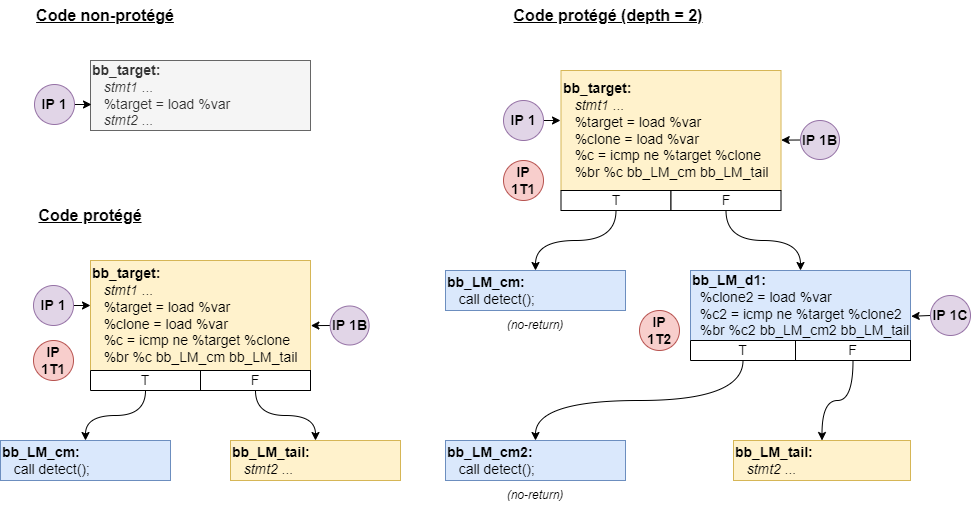
\includegraphics[scale=0.39]{ch5-placement/img/cm-mul-load-full-sep.drawio.png}
                    \caption{Schéma de protection de la multiplication de load}
                    \label{fig:lm-scheme}
                \end{figure}
            
                \begin{defi}
                    \label{def:cm-ponderated}
                    Une contre-mesure locale est dite \textit{pondérée} s'il est possible de l'appliquer avec une profondeur $p$ positive.
                    On note $C_p(P, IP)$ l'application d'une contre-mesure locale pondérée $C$ sur un point d'injection $IP$ avec une profondeur $p \in \mathbb{N}$.
                \end{defi}
                
                Ainsi, la \textit{duplication de test} correspond à une \textit{multiplication de test} de profondeur $1$.
                La figure \ref{fig:tt-scheme} présente le schéma de transformation de la multiplication de tests pour une profondeur $2$ (\gls{TT}). 
                Les points d'injection sont indiqués dans les cercles rouges à côté de l'instruction de branchement correspondante.
                La multiplication de tests peut être vue comme l'application successive de duplications de tests sur les points d'injection introduits par l'itération précédente, en ignorant la protection des branches allant vers un bloc de détection (c'est-à-dire contenant un appel à \textit{detect()} dans les schémas de protection présentés).        
                
                Les contre-mesures locales pondérées peuvent être appliquées avec une profondeur variable sur chaque point d'injection.
                L'intérêt de tels schémas dépend du fait qu'une application de profondeur $n+1$ apporte plus de garanties de sécurité qu'une application de profondeur $n$, pour un modèle de faute $m$, ce qu'on va pouvoir quantifier dans la suite de ce chapitre.
            
            \subsubsection{Multiplication de loads}
            \label{sec:cm-load-mult}
            
                La multiplication de tests vise le modèle de l'inversion de test (\gls{TI}). La multiplication de loads (\gls{LM}) est une contre-mesure locale pondérée visant le modèle de la mutation de données lors les \textit{loads} (\gls{DL}).
                
                La figure \ref{fig:lm-scheme} présente le schéma de protection de la multiplication de loads avec une profondeur $0$ (code non protégé), $1$ (\gls{LD}) et $2$ (\gls{LT}).
                Les points d'injection en rouge correspondent au modèle de faute \gls{TI} tandis que les violets correspondent au modèle \gls{DL}.
                Les blocs de base en jaune indiquent des blocs comportant à la fois des instructions du programme original et du code de contre-mesure.
                Dans le cas de la protection de profondeur 1, l'instruction \texttt{load} est dupliquée et les deux valeurs sont comparées. Si celles-ci sont différentes, le programme est arrêté, sinon le flot de contrôle revient à l'instruction suivant le \texttt{load} ciblé (ici dans un nouveau bloc \texttt{bb\_LM\_tail}). 
                Dans le cas de protection de profondeur 2 ou plus, comme indiqué dans la partie droite de la figure, les \texttt{load}s dupliqués sont comparés à la valeur du \texttt{load} original, générant ainsi plusieurs branchements conditionnels successifs.
            
        \subsection{Adéquation et coefficient de protection}
        \label{sec:cm-perfection}
        
            Cette section s'intéresse à la propriété d'adéquation d'une contre-mesure, définie par rapport à un modèle de faute.
            Cette propriété est nécessaire pour établir des garanties de robustesse pour les différents algorithmes de placement.
            La section \ref{sec:ooc} présente une approche d'analyse de contre-mesures \textit{en isolation}, visant à étudier les propriétés du schéma de protection en dehors d'un programme particulier.
            La section \ref{sec:fscenario} détaille le cas d'une analyse dans le scénario où une entrée est déjà corrompue.
            La section \ref{sec:cm-perfect} définit l'adéquation d'une contre-mesure locale à l'aide de cette analyse.
            
            \subsubsection{Analyse en isolation de schémas de protection}
            \label{sec:ooc}
            
                L'approche présentée ici consiste à s'intéresser aux comportements d'un schéma de protection en isolation, relativement à un modèle de faute.
                L'idée est d'explorer tous les chemins d'exécution fautée en prenant pour entrée le point d'injection (ici une instruction \gls{llvm}) en fonction du modèle de faute $m$ 
                afin de déterminer le nombre de fautes nécessaires pour le corrompre, appelé \textit{coefficient de protection} (définition \ref{def:cm-k}).
                Puisqu'un point d'injection est par définition attaquable en une faute, un schéma de protection avec $K > 1$ apporte des garanties sur la robustesse du schéma de protection.
                
                \begin{defi}
                    \label{def:cm-k}
                    Soit $S$ un schéma de protection sur un point d'injection, on appelle \textit{coefficient de protection} $K$ le nombre minimum de fautes nécessaires pour produire un comportement incorrect, pour un modèle de faute donné.
                \end{defi}     
                
                L'analyse en isolation d'un schéma de protection pour un modèle de faute $m$ nécessite de déterminer :
                \begin{itemize}
                    \item Les \textit{points d'entrée} et les \textit{points de sortie} du schéma de protection.
                    \item Les \textit{entrées} du schéma de protection.
                    \item Les \textit{sorties} du schéma de protection.
                    \item La \textit{surface d'attaque} du schéma de protection par rapport au modèle $m$.
                \end{itemize}

                \paragraph{}
                \textbf{Points d'entrée et de sortie.} Les \textit{points d'entrée et de sortie} sont définis par le schéma de protection, mais également par le modèle de faute $m$. Pour un modèle de faute de saut par exemple, l'exploration exhaustive des comportements du schéma de protection nécessite de prendre en compte comme points d'entrée chaque point d'arrivée de saut possible et comme points de sortie les points d'injection de saut.
                Les schémas de \gls{LM} et \gls{TM} (voir figure \ref{fig:td-scheme}, \ref{fig:tt-scheme} et \ref{fig:lm-scheme}) ne contiennent qu'un seul point d'entrée correspondant à l'instruction sur laquelle le schéma de protection s'applique (respectivement \texttt{br} et \texttt{load}).
                Le schéma \gls{LM} n'a qu'un seul point de sortie (le bloc \texttt{bb\_LM\_tail}) tandis que \gls{TM} en possède deux (les blocs cibles \texttt{bb\_true} et \texttt{bb\_false}).
                Notez qu'on ne considère pas les blocs de détection comme des points de sorties.
                
                \textbf{Entrées.} Les \textit{entrées} correspondent à tout état du programme qui est utilisé par le schéma de protection. Dans le cadre de la contre-mesure \gls{TM}, l'unique entrée est la valeur de condition \texttt{\%cond}, utilisée par les instructions de branchement.
                Pour la contre-mesure \gls{LM}, l'unique entrée est la valeur de la variable lue par les instructions \texttt{load}.
                
                \textbf{Sorties.} Les \textit{sorties} correspondent aux états du programme qui sont susceptibles d'être modifiés par le schéma de protection.
                Pour \gls{TM}, il s'agit du bloc d'arrivée ($bb\_true$ ou $bb\_false$). Pour \gls{LM}, la sortie correspond à la valeur lue par l'instruction \texttt{load}\footnote{C'est à dire la valeur qui sera stockée dans le registre temporaire \gls{llvm} $\%target$.}. 
                Les sorties sont nécessaires pour déterminer l'objectif d'attaque de l'analyse en isolation, une attaque réussie du schéma \gls{TM} correspondant à un branchement vers la mauvaise branche en sortie et pour \gls{LM} au chargement de la mauvaise valeur lors du load (sans qu'aucune fonction \texttt{detect} ne soit déclenchée).
                Il est possible d'avoir plusieurs sorties si on considère des contre-mesures avec \textit{état}, telles que \textit{SecSwift CF} \cite{Ferriere/LLVM19} citée précédemment.
                
                \textbf{Surface d'attaque.} La \textit{surface d'attaque} du schéma de protection correspond à tous les points d'injection du modèle $m$, que ce soit le point d'injection nominal (celui sur lequel le schéma s'applique) mais aussi les points d'injection introduits par la contre-mesure.
                
                \begin{defi}[Surface d'attaque]
                    \label{def:cm-ips}
                    Soit $C$ une contre-mesure et $IP$ un point d'injection, on note $IPs(C(P, IP))$ l'ensemble des points d'injection introduits par l'application $C(P, IP)$.
                \end{defi}
                    
                \begin{figure}[p]\centering
            \begin{multicols}{2} 

\lstset{language=C,style=codeC, caption={Encodage de $TD$ ($TM_1$)},label={lst:td-scheme-lazart}, showlines=true}
\begin{lstlisting}
int tm_scheme(int cond) {
    bb_start:
    if(cond) {
        bb_TM_1T:
        if(cond) {
            bb_true:
            return true;
        } else {
            bb_cm1T:
            detect();
        }
    } else {
        bb_TM_1F:
        if(cond) {
            bb_cm1F:
            detect();
        } else {
            bb_false:
            return false;
        }
    }
}













\end{lstlisting}  
\columnbreak

\lstset{language=C,style=codeC, caption={Encodage de $TT$ ($TM_2$)},label={lst-tt-scheme-lazart}, showlines=true}
\begin{lstlisting}
int tm_scheme(int cond) {
    bb_start:
    if(cond) {
        bb_TM_1T:
        if(cond) {
            bb_TM_2T:
            if(cond) {
                bb_true:
                return true;
            } else {
                bb_cm2T:
                detect();
            }
        } else {
            bb_cm1T:
            detect();
        }
    } else {
        bb_TM_1F:
        if(cond) {
            bb_cm1F:
            detect();
        } else {
            bb_TM_2T:
            if(cond) {
                bb_cm2F:
                detect();
            } else {
                bb_false:
                return false;
            }
        }
    }
}

\end{lstlisting} 
\end{multicols}
            \end{figure}

\begin{figure}[p]\centering
\lstset{caption={Fonction principale de l'analyse en isolation (scénario nominal)},label=lst:ooc-main-lazart}
\begin{lstlisting}
int main() {
    int entry;
    klee_make_symbolic(&entry, sizeof(entry), "cond");

    int br = tm_scheme(entry);

    _LZ__ORACLE((br != (entry ? true : false)));
}
\end{lstlisting}
            \end{figure}
        
                A partir de ces quatre paramètres, il est possible d'explorer les exécutions fautées du schéma de protection. Cette exploration peut être effectuée avec Lazart\footnote{Le nombre de chemins à explorer dans une analyse en isolation est généralement petit. Ainsi, il est possible de vérifier manuellement que l'exploration symbolique est correcte et complète.}, comme montré dans les listings \ref{lst:td-scheme-lazart} et \ref{lst-tt-scheme-lazart} qui correspondent à l'encodage en langage C des schémas de protection de la multiplication de tests, respectivement pour une profondeur de $1$ et de $2$.
                Les noms des blocs de base (correspondant à ceux des figures \ref{fig:td-scheme} et \ref{fig:tt-scheme}) sont indiqués en tant qu'étiquettes (labels ).
                L'entrée du schéma de protection est représentée par l'entier \texttt{cond} et la branche de sortie est représentée sous la forme d'un booléen (branche \textit{true} ou branche \textit{false}).
                Les appels à \texttt{detect()} correspondent à une détection de l'attaque.
        
                Le listing  \ref{lst:ooc-main-lazart} correspond à la fonction principale de l'analyse avec Lazart.
                La condition d'entrée est déclarée comme variable symbolique (ligne 3) et l'objectif d'attaque consiste à retourner la mauvaise branche (vérifié ligne 7).
                La recherche des chemins d'attaque est effectuée en fautant la fonction correspondant au schéma de protection (ici \texttt{tm\_scheme}) avec le modèle $m$ (ici \gls{TI}).

                La table \ref{tbl:tm-ooc-N} présente les résultats de l'analyse en isolation pour différentes profondeurs de protection de la multiplication de tests.
                La colonne "Contre-mesure" indique le schéma de protection: $P$ correspondant à une profondeur 0 (code non protégé), \gls{TD} à la duplication de test (\gls{TM} profondeur 1) et \gls{TT} à la triplication de test (\gls{TM} de profondeur 2).
                Les colonnes suivantes indiquent le nombre d'attaques trouvées pour chaque nombre de fautes et la dernière colonne "$K_n$" correspond au \textit{coefficient de protection nominal}, c'est-à-dire le nombre minimum de fautes nécessaires pour valider l'objectif d'attaque.
    
                \begin{table}[ht]
                    {\small
                    \begin{center}
                        \begin{tabular}{l|cccccc}
                        Contre-mesure & 0 faute & 1 faute & 2 fautes & 3 fautes & 4 fautes & $K_n$ \\
                        \hline
                        $TM_0$ ($P$) & 0 & 1 & 0 & 0 & 0 & 1\\
                        $TM_1$ ($TD$) & 0 & 0 & 1 & 0 & 0 & 2 \\
                        $TM_2$ ($TT$) & 0 & 0 & 0 & 1 & 0 & 3
                        \end{tabular}
                    \end{center} 
                    }
                    \caption{Évaluation en isolation de $TM$ \label{tbl:tm-ooc-N}}
                \end{table}
            
            \subsubsection{Scénario corrompu}
            \label{sec:fscenario}
            
                Afin d'être exhaustif sur l'exploration des comportements, il est nécessaire de se pencher sur le cas où les entrées de la contre-mesure sont déjà corrompues (par une faute précédente).
                Ainsi, la méthodologie d'analyse en isolation distingue deux scénarios, comme indiqué dans la figure \ref{fig:out-of-context}:
                \begin{itemize}
                    \item Scénario Nominal (N) : toutes les entrées sont saines (traité dans la section précédente).
                    \item Scénario Corrompu (C) : une entrée au moins est corrompue en amont du schéma de protection.
                \end{itemize}
                
                \begin{table}[ht]
                    {\small
                    \begin{center}
                        \begin{tabular}{l|cccccc}
                        Contre-mesure & 0 faute & 1 faute & 2 fautes & 3 fautes & 4 fautes & $K_c$ \\
                        \hline
                        $TM_0$ ($P$) & 1 & 0 & 0 & 0 & 0 & 0\\
                        $TM_1$ ($TD$) & 1 & 0 & 0 & 0 & 0 & 0\\
                        $TM_2$ ($TT$) & 1 & 0 & 0 & 0 & 0 & 0
                        \end{tabular}
                    \end{center} 
                    }
                    \caption{Évaluation en isolation de $TM$ (scénario corrompu)\label{tbl:tm-ooc-F}}
                \end{table}
                      
                \begin{figure}[!htp]\centering
                    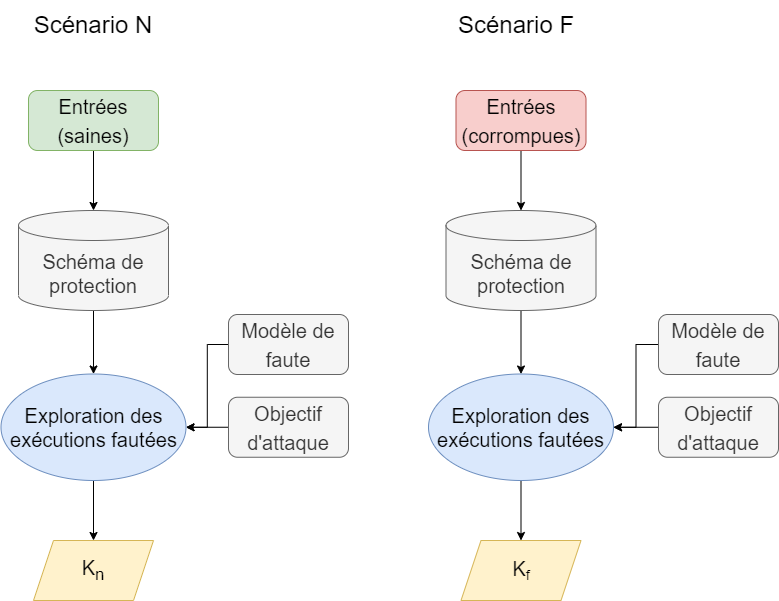
\includegraphics[scale=0.39]{ch5-placement/img/out-of-context-metho.png}
                    \caption{Évaluation de schéma de protection en isolation}
                    \label{fig:out-of-context}
                \end{figure}
        
                La table \ref{tbl:tm-ooc-F} présente les résultats (après analyse de redondance-équivalence) du scénario corrompu (C) pour l'exemple précédent, la condition d'entrée étant falsifiée (en changeant donc l'appel ligne 5 en \texttt{int br = tm\_scheme(!entry);}\footnote{Dans le cas d'une entrée non booléenne, celle-ci serait contrainte comme étant différente de la valeur nominale (\texttt{\_LZ\_\_ORACLE(entry != expected\_value);}.}). 
                On appellera respectivement \textit{coefficient de protection nominal} ($K_n$) et \textit{coefficient de protection corrompu} ($K_c$) les coefficients de protection obtenus pour respectivement les scénarios $N$ et $C$.
                Pour les contre-mesures \gls{TM} et \gls{LM} et leurs modèles de faute respectifs \gls{TI} et \gls{DL} avec une pondération d'application $p$, on obtient $K_n = 1 + p$ et $K_c = 0$. 
                Cela implique que, si les entrées d'un schéma de protection \gls{TM} ou \gls{LM} sont nominales, alors on a la garantie que le programme sera dans un état nominal en sortie du schéma de protection en moins de $1 + p$ fautes injectées localement. 
                En revanche, dans le scénario corrompu, tous les schémas de protection produisent un comportement incorrect même en l'absence de faute, de la même manière que le point d'injection non protégé.
                
            \subsubsection{Adéquation des contre-mesures}
            \label{sec:cm-perfect}
        
                \begin{defi}[Adéquation]
                    \label{def:cm-pperfect}
                    Pour un modèle de faute $m$, une contre-mesure locale $C$ est dite \textit{adaptée} ssi, pour tout programme $P$, son coefficient de protection nominal $K_n$ est strictement supérieur à 1.
                \end{defi}
                
                \begin{defi}[Perfection]
                    \label{def:cm-perfect}
                    Pour un modèle de faute $m$, une contre-mesure locale $C$ est dite \textit{parfaite} ssi, pour tout programme $P$, son coefficient de protection $K = min(K_n, K_c)$ est strictement positif. 
                \end{defi}
                
                Une contre-mesure parfaite (définition \ref{def:cm-perfect}) garantit que, quelles que soient les entrées d'une contre-mesure, tout état invalide du programme sera détecté. 
                La section \ref{sec:model-protectability} revient sur l'existence de telles contre-mesures, mais on peut observer que ce n'est pas le cas des contre-mesures \gls{TM} et \gls{LM}, qui ont $K_c$ nul. En effet, si les entrées sont déjà corrompues, alors le comportement du point d'injection protégé restera incorrect (mauvaise branche ou valeur incorrecte) sans qu'aucune faute ne soit injectée.
                En revanche, \gls{TM} et \gls{LM} sont des contre-mesures adaptées (définition \ref{def:cm-pperfect}) pour respectivement les modèles \gls{TI} et \gls{DL} (propriétés \ref{hypo:test-mult} et \ref{hypo:load-mult}).
                Comme cela a été expliqué dans la section précédente, l'analyse en isolation avec l'exécution symbolique (via Lazart) génère peu de chemins pour nos exemples et il est donc possible de vérifier la complétude de l'exploration des chemins manuellement. 
                La preuve de la propriété d'adéquation d'un schéma de protection par rapport à un modèle de faute pourrait aussi être effectuée à l'aide d'un outil d'analyse statique ou d'un assistant de preuve.
                
                \begin{proper}
                    \label{hypo:test-mult}
                    La multiplication de tests est une contre-mesure locale pondérée adaptée pour le modèle de l'inversion de test (\gls{TI}).
                \end{proper}
            
                \begin{proper}
                    \label{hypo:load-mult}
                    La multiplication de loads est une contre-mesure locale pondérée adaptée pour le modèle de la mutation de données sur les loads (\gls{DL}).
                \end{proper}
                
        \subsection{Complétude d'une contre-mesure et catalogue}
        \label{sec:cm-complete}
         
            Les contres-mesures \gls{TM} et \gls{LM} sont chacune des contres-mesures adaptées pour respectivement les modèles \gls{TI} et \gls{DL}. 
            \gls{TM} et \gls{LM} sont aussi adaptées pour le modèle combiné de l'inversion de test et de la mutation de données ($TI+DL$).
            En effet, chacune a un coefficient de protection nominal $K_n$ strictement supérieur à 1 lorsqu'on les étudie en fonction du modèle $m = TI+DL$.
            
            Néanmoins, ni \gls{TM}, ni \gls{LM}, ne permettent indépendamment la protection de l'ensemble des points d'injection du modèle $TI+DL$. On dit alors que chacune de ces contre-mesures sont \textit{incomplètes} pour le modèle $TI+DL$ (définition \ref{def:cm-compl}).
            Ainsi, on appellera \gls{TLM} la contre-mesure locale pondérée correspondant à l'application de \gls{TM} sur les points d'injection \gls{TI} et \gls{LM} pour les points d'injection \gls{DL}. Cette contre-mesure est complète et adaptée pour le modèle $TI+DL$ (propriété \ref{hypo:tl-mult}).
            
            \begin{defi}
                \label{def:cm-compl}
                Une contre-mesure locale est dite \textit{complète} pour un modèle de faute $m$, si elle propose une schéma de protection pour tous les points d'injection générés par le modèle de faute $m$.
            \end{defi}
        
            \begin{proper}
                \label{hypo:tl-mult}
                La multiplication de tests et de loads (\gls{TLM}) est une contre-mesure locale pondérée adaptée et complète pour le modèle $TI+DL$.
            \end{proper}

            Les algorithmes de placement qui seront présentés par la suite considèrent un \textit{catalogue} de contre-mesures.
            Ce catalogue associe un schéma de protection en fonction d'un point d'injection suivant son modèle de faute et un coefficient de protection.
            \gls{TLM} peut être vu comme un catalogue de contre-mesure associant \gls{TM} aux points d'injection \gls{TI} et \gls{LM} aux points d'injections \gls{DL}, le schéma de protection précis qui sera retourné dépendant du coefficient de protection demandé\footnote{Par exemple, pour un point d'injection \gls{TI} et un coefficient de protection de $2$, le catalogue retournerait la duplication de test.}.            
            Les notions d'adéquation et de complétude peuvent être étendues à un catalogue de contre-mesures (définitions \ref{def:catalog-adatp} et \ref{def:catalog-complete}).
            Les algorithmes de placement présentés par la suite considèrent les catalogues totaux\footnote{Un catalogue total est complet et adapté.} (définition \ref{def:catalog-pond-adatp}).
            
            \begin{defi}[Catalogue adapté]
                \label{def:catalog-adatp}
                Un catalogue de contre-mesures $\mathcal{C}$ est adapté pour un modèle de faute $m$, si toutes les schémas de protection sont adaptés pour le modèle $m$.
            \end{defi}
            
            \begin{defi}[Catalogue complet]
                \label{def:catalog-complete}
                Un catalogue de contre-mesures $\mathcal{C}$ est complet pour un modèle de faute $m$, s'il associe un schéma de protection pour tous les points d'injection du modèle de faute $m$.
            \end{defi}
            
            \begin{defi}[Catalogue total]
                \label{def:catalog-pond-adatp}
                Un catalogue de contre-mesures $\mathcal{C}$ est dit total pour un modèle de faute $m$, s'il possède un schéma de protection pour tout points d'injection et pour tout coefficient de protection $k$, avec $1 \leq k \leq n+1$, pour $m$, avec $n \in \mathbb{N}^*$.
            \end{defi}

            Un catalogue de contre-mesures n'est donc finalement qu'une forme particulière de contre-mesure, permettant de garantir qu'un point d'injection est protégé qu'une fois par un schéma de protection (quelle que soit la profondeur d'application choisie).
            De cette manière, plusieurs contre-mesures (de l'ordre du point d'injection) qui ne sont pas indépendantes peuvent être appliquées de manière indépendante.
            En effet, les contre-mesures \gls{TM} et \gls{LM} ne sont pas indépendantes. \gls{LM} introduit des points d'injections \gls{TI} qui peuvent ainsi être protégés par une application de \gls{TM} (en d'autres termes, $TM(LM(P)) \neq LM(TM(P))$).
            Il est donc nécessaire de s'assurer qu'un point d'injection ne soit pas protégé plusieurs fois de manière à garantir l'indépendance de l'application.
                    
        \subsection{Synthèse}
        \label{sec:cm-synthesis}
        
            La table \ref{tbl:local-cm-comparison} présente un résumé des caractéristiques des différentes contre-mesures abordées dans cette section. La colonne "CM" indique le nom de la contre-mesure.
            Les colonnes "Adéquation" et "Complétude" indiquent respectivement si la contre-mesure est adaptée et complète, par rapport aux différents modèles de faute. Pour la complétude, la valeur "-" indique que la contre-mesure ne permet de protéger aucun point d'injection du modèle de faute.
            La colonne "Surface d'attaque" indique le nombre de points d'injection générés par la contre-mesure pour une profondeur $p$ respectivement pour les modèles \gls{TI} et \gls{DL} (c'est-à-dire $IPs(C_p(P, IP))$).
            Ces valeurs ne sont pas indiquées pour \gls{TLM} puisqu'elle correspond à celles de \gls{TM} ou \gls{LM} en fonction du modèle du point d'injection protégé.
            
            \begin{table}[h]
                {\small
                \begin{center}
                    \begin{tabular}{c|ccc|ccc|cc}
                    CM & \multicolumn{3}{c|}{Adéquation} & \multicolumn{3}{c|}{Complétude} & \multicolumn{2}{c}{Surface d'attaque}  \\
                    \multicolumn{1}{l|}{} & TI & DL & TI+DL & TI & DL & TI+DL & TI & DL  \\
                    \hline
                    \gls{TM} & Oui & Oui & Non & Oui & - & Non & $2p$ & $0$  \\
                    \gls{LM} & Oui & Oui & Non & - & Oui & Non & $p$ & $1 + p$ \\
                    \gls{TLM} & Oui & Oui & Oui & Oui & Oui & Oui & - & - 
                    \end{tabular}
                \end{center} 
                }
                \caption{Comparaison des contre-mesures locales pondérées\label{tbl:local-cm-comparison}}
            \end{table}
        
            Les notions de contre-mesures \textit{locales} et \textit{pondérées} sont nécessaires pour les algorithmes de placement.
            Ces contre-mesures peuvent être représentées par l'ensemble des pondérations associées à chaque point d'injection de fautes du programme, une pondération de 0 correspondant à ne pas protéger le point d'injection. 
            Si on considère des contre-mesures locales mais non pondérées (\gls{CL}), leur application est aussi un ensemble de pondérations dont les valeurs sont comprises entre 0 et 1.
            Enfin, dans le cas de contre-mesures à granularité du point d'injection mais non indépendantes (C), alors l'ordre dans lequel les protections sont appliquées est important. Dans ce cas, l'application de la contre-mesure peut être représentée par une liste ordonnée de points d'injection à protéger.
            Les notions d'\textit{adéquation} et de \textit{complétude} sont quant à elles utiles pour déterminer les garanties en terme de robustesse pour un algorithme de placement. 
            
            \begin{table}[htp]
                {
                \begin{center}
                    \begin{tabular}{l|cc}
                    Contre-mesure & Acronyme & Autre nom \\
                    \hline 
                    Multiplication de tests & $TM$ & - \\
                    $\;\;$ Duplication de tests & $\;TD$ & $\;TM_1$ \\
                    $\;\;$ Triplication de tests & $\;TT$ & $\;TM_2$ \\
                    Multiplication de loads & $LM$ & - \\
                    $\;\;$ Duplication de loads & $\;LD$ & $\;LM_1$ \\
                    $\;\;$ Triplication de loads & $\;LT$ & $\;LM_2$ \\
                    \begin{tabular}[c]{@{}l@{}}Multiplication de loads\\ et de tests\end{tabular} & $TLM$ & -
                    \end{tabular}
                \end{center} 
                }
                \caption{Abréviation pour les différentes contre-mesures locales de Lazart\label{tbl:cm:nomenclature}}
            \end{table}
            
            \begin{table}[htp]
                {\small
                \begin{center}
                    \setlength\tabcolsep{5pt}
                    \begin{tabular}{l|cccc}
                    Localité / Pondération & \multicolumn{4}{c}{Adéquation / Complétude} \\
                     & Inadaptée (-I) & Adaptée (-A) & Complète (-C) & Parfaite (-P) \\
                     \hline
                    CM non locale (C) & C-I & C-A & C-C & C-P \\
                    CM Locale (CL) & CL-I & CL-A & CL-C & CL-P \\
                    CM Locale Pondérée (CLP) & CLP-I & CLP-A & CLP-C & CLP-P
                    \end{tabular}
                \end{center} 
                }
                \caption{Abréviation pour les différentes catégories de contre-mesures à granularité IP\label{tbl:cm:nomenclature-types}}
            \end{table}
        
            Les tables \ref{tbl:cm:nomenclature} et \ref{tbl:cm:nomenclature-types} proposent un résumé des abréviations qui seront utilisées dans la suite de ce chapitre. La table \ref{tbl:cm:nomenclature} indique les abréviations utilisées pour les contre-mesures étudiées ici. La table \ref{tbl:cm:nomenclature-types} indique les abréviations concernant les différentes classes de contre-mesures. Par exemple, \gls{CLP}-AC correspond à une Contre-mesure Locale Pondérée, Adaptée et Complète (pour un modèle de faute donné).
            
    \section{Placement de contre-mesures adaptées}
    \label{sec:placement}

        L'approche de placement de contre-mesures présentée dans ce chapitre se base sur l'analyse en isolation des schémas de protections et sur une exploration des traces d'attaques réussies, par rapport à un modèle de faute et un objectif d'attaque.
        L'analyse en isolation fournit des garanties sur le comportement d'un point d'injection protégé, et les traces d'attaques permettent de déterminer quels sont les points d'injection à protéger.
        Les algorithmes présentés ici prennent ainsi en entrées:
        \begin{itemize}
            \item Le catalogue de contre-mesures $\mathcal{C}$.
            \item Le modèle d'attaquant $M = \{m, \phi\}$, avec $m$ le modèle de faute et $\phi$ l'objectif d'attaque.
            \item Le nombre de fautes $n$ pour lequel on souhaite être robuste.
        \end{itemize}

        Le catalogue $\mathcal{C}$ est un catalogue total (définition \ref{def:catalog-pond-adatp}) pour le modèle $m$.
        Les garanties de robustesse sont données en supposant que l'énumération des chemins d'attaque est \textit{correcte} et \textit{complète} (définitions \ref{def:fi-sound} et \ref{def:fi-complete}).
        Les algorithmes génèrent un programme $P'$ protégé dont les garanties dépendent de l'algorithme et du catalogue, et visent:
        \begin{itemize}
            \item La \textit{robustesse} du programme $P'$ en $n$ fautes.
            \item L'\textit{optimalité} du placement.
        \end{itemize}

        La section \ref{sec:placement-syst} présente trois algorithmes de placement systématique.
        La section \ref{sec:placement-bloc} décrit le placement par bloc, dans lequel seul un \gls{ip} par trace d'attaque est protégé.
        La section \ref{sec:placement-opti} traite du placement réparti où différents \gls{ip}s peuvent être protégés avec des coefficients de protection différents.
        Finalement, la section \ref{sec:placement-other} discute des garanties lorsque le catalogue ne dispose pas d'un schéma avec un coefficient de protection suffisant et discute de certaines variantes des algorithmes précédents.  
            
        \subsection{Placement systématique}
        \label{sec:placement-syst}

            Lorsqu'on s'intéresse à un catalogue total pour le modèle de faute $m$, appliquer un schéma de protection avec un coefficient de protection nominal $K_n = n+1$ sur tous les points d'injection garantit une robustesse en au moins $n$ fautes du programme protégé. 
            En effet, l'analyse en isolation garantit que le comportement du schéma de protection est nominal en moins de $n + 1$ fautes si les entrées sont nominales. Si tous les points d'injection sont protégés avec $K_n = n+1$, il faudra $n + 1$ fautes pour casser indépendamment chaque schéma et aucun schéma de protection ne pourra être corrompu en $n$ fautes.

            On distinguera trois versions de l'algorithme de placement systématique:
            \begin{itemize}
                \item Le placement systématique naïf (\texttt{naïf}): tous les points d'injection du programme sont protégés avec $K_n = n+1$.
                \item Le placement systématique sur les attaques (\texttt{atk}): tous les points d'injection intervenant au moins une fois dans une attaque sont protégés avec $K_n = n+1$.
                \item Le placement systématique sur les minimales (\texttt{min}): seuls les points d'injection intervenant dans les attaques minimales sont protégés avec $K_n = n+1$.
            \end{itemize}

            Si l'énumération des chemins fautés est correcte et complète, alors protéger les points d'injection intervenant dans les attaques est suffisant.
            De plus, la protection des attaques minimales est suffisante, puisque si une attaque $a'$ est redondante par rapport à une attaque $a$, protéger $a$ pour $n$ fautes implique que $a'$ sera robuste en $n+1$ fautes au minimum.

            Le listing \ref{lst:placement-syst} correspond au pseudo-code de l'algorithme de placement systématique sur les attaques minimales (\texttt{min}) prenant en entrées le catalogue $\mathcal{C}$, le programme $P$, le modèle d'attaquant $M$ et le nombre de fautes $n$ pour lequel le programme $P'$ doit être robuste.
            Les attaques minimales sont obtenues à partir d'une analyse d'attaque et une analyse de redondance (lignes 3 et 5) puis chaque point d'injection intervenant au moins une fois dans une attaque minimale se voit assigner un coefficient de protection de $n + 1$ (lignes 11 à 13).
            Le programme $P'$ est généré à partir de l'ensemble des coefficients de protection (lignes 16 à 19) en sélectionnant le schéma de protection à appliquer à partir du catalogue (représenté par la fonction \texttt{get\_cm} ligne 18).

\lstset{caption={Algorithme de placement systématique \texttt{min}},label=lst:placement-syst, showlines=true}
\begin{lstlisting}
def placement_min(C: Catalog, P: Program, M: AttackModel, n: int):
    # Get sucessfull non-detected attacks.
    attacks = T_s(P, M, n)
    # Filter with minimals attacks.
    minimals = RedundacyAnalysis(attacks).minimals()
    
    # Initial protection factors Kn at 1 for all IP.
    required_kn = { IPA: 1, IPB: 1, ..., IPN: 1 }

    # Apply ponderation of n for all IP in traces
    for attack in minimals:
        for IP in attack:
            required_kn[IP] = n + 1 # Make IP robust en n faults.

    # Generation of P'
    P` = P
    for IP, kn in required_kn:
        S = C.get_cm(IP.model(), kn) # Select protection scheme from catalog
        P` = S(P`, IP) # Apply local protection        
    return P`
\end{lstlisting}  

        \subsection{Placement par bloc}
        \label{sec:placement-bloc}

            L'algorithme de placement systématique sur les attaques minimales protège l'ensemble des points d'injection intervenant dans une attaque.
            L'algorithme de placement par bloc (\texttt{bloc-h}) présenté dans cette section vise à protéger au moins un point d'injection par attaque minimale, avec $K_n = n + 1$.

\lstset{caption={Algorithme de placement par bloc avec heuristique \texttt{bloc-h}},label=lst:placement-bloc-h, showlines=true}
\begin{lstlisting}
def placement_bloc_h(C: Catalog, P: Program, M: AttackModel, n: int):
    # Get sucessfull non-detected attacks.
    attacks = T_s(P, M, n)
    # Filter with minimals attacks.
    minimals = RedundacyAnalysis(attacks).minimals()
    
    # Initial protection factors Kn at 1 for all IP.
    required_kn = { IPA: 1, IPB: 1, ..., IPN: 1 }
            
    # For all attacks by faults count.
    for order in 1 to n:
        # Loop trought order-faults attacks by number of associated redundant attacks.
        for attack in minimals.where(order=order).sort_by(Minimals):
            if is_protected(attack, required_kn):
                continue
            # Make attack robust in n faults
            IP = select IP in attack with most occurence
            required_kn[IP] = n

    # Generation of P'
    P` = P
    for IP, kn in required_kn:
        S = C.get_cm(IP.model(), kn) # Select protection scheme from catalog
        P` = S(P`, IP) # Apply local protection        
    return P`
\end{lstlisting}  

            Le listing \ref{lst:placement-bloc-h} présente le pseudo-code de l'algorithme de placement par bloc avec heuristiques. 
            Pour chaque nombre de fautes, toutes les attaques minimales sont parcourues.
            Si une attaque n'est pas protégée (c'est-à-dire qu'il n'y a pas au moins un \gls{ip} protégé au niveau $n$, vérifié par la fonction \texttt{is\_protected} ligne 14), un \gls{ip} est sélectionné pour être protégé (ligne 17).
            La pondération de protection obtenue dépend ainsi de deux leviers :
            \begin{itemize}
                \item \textit{l'ordre dans lequel les traces sont protégées} : l'algorithme utilise une heuristique consistant à parcourir les attaques minimales uniquement, par ordre de leur nombre de fautes, et par nombre de traces redondantes associées ($Red(a)$) décroissant \footnote{C'est-à-dire que si deux traces ont le même nombre de fautes et sont minimales, on privilégiera les attaques avec le plus grand nombre d'attaques redondante associées.}. 
                \item \textit{le point d'injection sélectionné lors de la protection d'une attaque} : ici l'heuristique consiste à sélectionner les \gls{ip}s en fonction de leur nombre d'occurrences dans l'attaque considérée, puis en fonction de leur nombre de déclenchements total au sein des attaques minimales (obtenu à l'aide d'une analyse de point chauds, voir section \ref{sec:hotspots}).  
            \end{itemize}
            
            Dans le cas du placement par bloc, protéger un \gls{ip} avec un coefficient de protection $n+1$ dans chaque attaque garantit que chaque attaque nécessitera au moins $n + 1$ fautes pour être réussie.
            Toute attaque en moins de $n + 1$ fautes sera soit bloquée par un \gls{ip} protégé, soit une attaque non réussie (les sorties produites par l'\gls{ip} protégé étant nominales), ce qui est garanti par l'exploration des chemins d'exécution fautés de $P$.

        \subsection{Placement réparti}
        \label{sec:placement-opti}

            Le placement par bloc présenté précédemment impose la protection avec un coefficient de protection $K_n = n + 1$ pour au moins un \gls{ip} par trace d'attaque minimale.
            Le placement réparti s'autorise à protéger avec $K_n < n + 1$ les \gls{ip}s, de manière à répartir les protections sur plusieurs \gls{ip}s.
    
            La section \ref{sec:placement-isolation} explique pourquoi le placement peut être réparti dans une attaque sans risquer d'introduire des nouveaux chemins d'attaque.
            La section \ref{sec:placement-optimal-ilp} ramène la problématique du calcul optimal du placement réparti à un problème d'optimisation linéaire en nombre entier.
            Finalement, la section \ref{sec:placement-optimal-algo} présente l'algorithme de placement réparti optimal.
        
            \subsubsection{Protection des traces d'attaque}
            \label{sec:placement-isolation}
    
                La figure \ref{fig:placement-isol} présente le principe de la combinaison de l'analyse en isolation et l'exploration des traces d'attaques.
                Les blocs "IP X" correspondent aux déclenchements de fautes sur un \gls{ip} X.
                L'analyse en isolation (en haut) vise à abstraire les comportements possibles d'un point d'injection, que celui-ci soit protégé ou non. Tous les différents chemins ajoutés par la protection du point d'injection sont explorés dans l'analyse en isolation, permettant de déterminer combien de fautes doivent être dépensées pour obtenir une sortie invalide.  
                Dans l'exemple présenté sur la figure \ref{fig:placement-isol}, deux chemins existent pour l'\gls{ip} non protégé (à gauche): le chemin d'exécution nominale produisant une sortie nominale (en vert) et le chemin fauté produisant une sortie invalide (en rouge).
                Pour la version protégée avec $K_n = 2$ (à droite), l'attaque de $IP_{B2}$ introduit par la contre-mesure permet d'obtenir un comportement fauté en deux fautes (le chemin avec une seule faute étant bloqué).
    
                \begin{figure}[ht]\centering
                    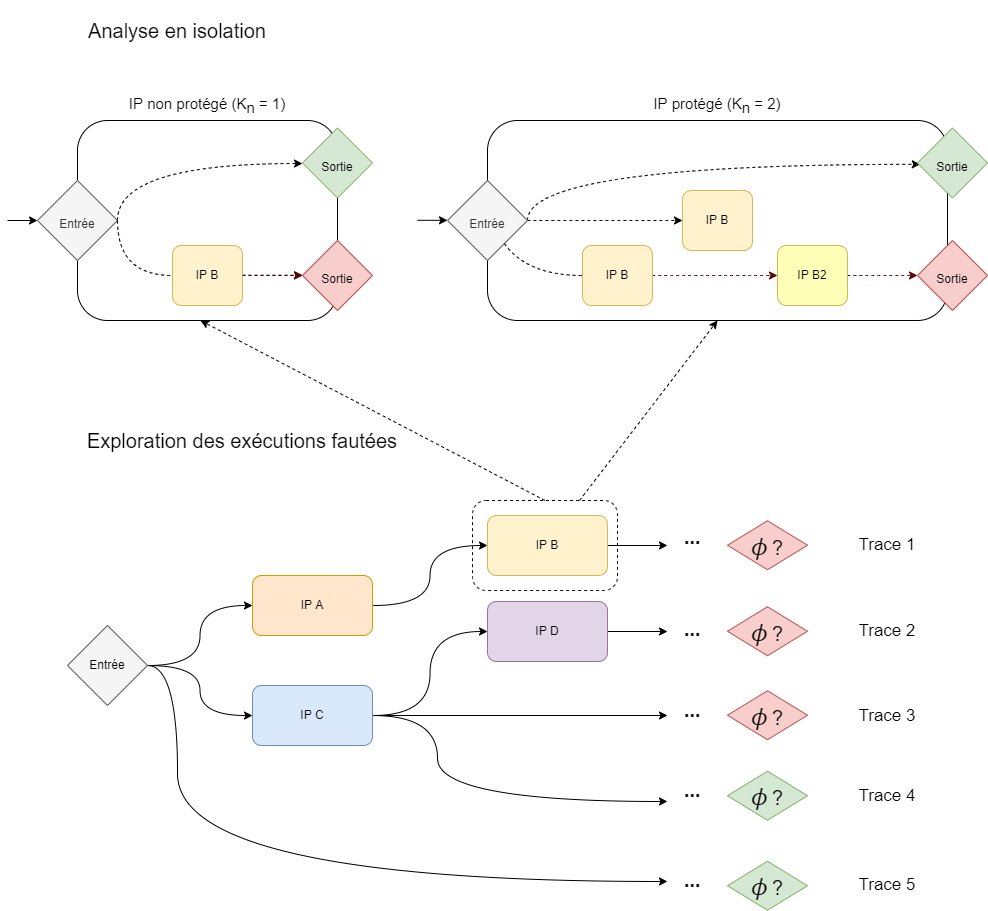
\includegraphics[scale=0.39]{ch5-placement/img/placement-isolation.drawio.png}
                    \caption{Principe général du placement avec analyse en isolation}
                    \label{fig:placement-isol}
                \end{figure}
            
                L'exploration des traces d'attaque donne des informations sur les relations entre les entrées et les sorties des différents points d'injection.   
                L'objectif est de déterminer si un \gls{ip} peut être protégé partiellement (avec un coefficient de protection inférieur à $n + 1$), sans que la sortie invalide qu'il produira n'introduise de nouveaux chemins fautés qui n'auraient pas été pris en compte.            
                Dans la figure \ref{fig:placement-isol}, l'exploration des chemins fautés (en bas), contient des informations sur les effets possibles d'une sortie corrompue d'un point d'injection. Les losanges verts indiquent que l'objectif d'attaque n'est pas validé (attaque non réussie), et les losanges rouges indiquent une attaque réussie.
                
                Par exemple, si on s'intéresse à la trace $2$, comportant la séquence de points d'injection déclenchés $\{ IP_C, IP_D \}$, on peut déterminer qu'un coefficient de protection de $3$ pour $IP_C$ serait suffisant pour obtenir une robustesse en 3 fautes\footnote{Pour $K_n = 3$, la Trace $4$ deviendrait une attaque en $4$ fautes, une faute étant nécessaire pour casser le point d'injection $IP_D$ non protégé.}.
                On peut alors se poser la question de si une attaque en 3 fautes est possible après la sortie invalide de l'\gls{ip} $IP_C$, qui ne demande que 3 fautes pour être corrompue.
                La réponse est donnée par l'exploration complète des traces d'attaques. La trace $4$ est une attaque non réussie et n'est donc pas à prendre en compte.
                En revanche la trace $3$ indique que si $IP_C$ n'est protégé qu'avec un coefficient de protection de $3$, alors la sortie invalide de $IP_C$ peut produire une attaque en $3$ fautes. Un coefficient de protection d'au moins $4$ est nécessaire sur $IP_C$ pour garantir la robustesse en 3 fautes.
    
                L'objectif est de pouvoir substituer les comportements des \gls{ip}s protégés à ceux des \gls{ip}s non protégés qui sont analysés dans l'exploration des exécutions fautées sur $P$, de manière à pouvoir prévoir comment un \gls{ip} protégé va se comporter dans le contexte du programme. 
                L'analyse en isolation abstrait les comportements fautés dans l'\gls{ip}, mais il est nécessaire de garantir que les comportements produits par un point d'injection fauté sont bien inclus dans les modèles de faute utilisés dans l'exploration préliminaire des exécutions fautées. 
                Dans le cadre des modèles de faute \gls{TI} et \gls{DL}, les sorties invalides d'un \gls{ip} fautés sont en effet incluses dans les modèles de Lazart:
                \begin{itemize}
                    \item Pour \gls{TI}, les différents schémas de protection de \gls{TM} peuvent produire une sortie vers la mauvaise branche.
                    \item Pour \gls{DL}, les différents schémas de protection de \gls{LM} peuvent produire une valeur erronée lue par le \texttt{load}, qui correspond au modèle \gls{DL}.
                \end{itemize}
    
                Ce ne serait pas le cas avec tous les modèles. Par exemple une mutation de donnée en mise-à-zéro, pourrait potentiellement produire des comportements différents (comme une mise-à-un) en fonction du schéma de protection.
                Pour garantir la possibilité de substituer les \gls{ip} protégés et non protégés, il serait nécessaire de montrer que les schémas de protection ne peuvent produire que le comportement nominal ou des mises-à-zéro, ou bien utiliser un modèle de mutation de donnée général (symbolique) dans l'exploration des chemins fautés afin de garantir cette inclusion.
     
            \subsubsection{Un problème d'optimisation linéaire}
            \label{sec:placement-optimal-ilp}
    
                La recherche des meilleurs placements répartis (dont le total des pondérations de protection appliquées et minimal) correspond à la recherche des ensembles de coefficients de protection minimaux tels que toute attaque réussie dans $T(P', M)$ nécessite au moins $n + 1$ fautes. 
                L'idée est de couvrir toutes les attaques, chaque attaque donnant un ensemble de contraintes sur les coefficients de protection à appliquer à chaque \gls{ip} pour obtenir la garantie de robustesse. On peut notamment remarquer:
                \begin{itemize}
                    \item si plusieurs \gls{ip}s apparaissent dans une attaque, alors chaque \gls{ip} peut être protégé indépendamment pour obtenir au final une attaque en plus de $n$ fautes.
                    \item si un point d'injection $ip$ apparaît $x$ fois dans une attaque, alors une protection sur $ip$ ajoute la nécessité de $x*K_n$ fautes supplémentaires.
                \end{itemize}        
        
                Les contraintes imposées par une attaque $a$ peuvent se traduire par une inégalité $C_a$ de la forme $\alpha x_1 + ... + \gamma x_n \geq n + 1$, avec $n$ le nombre de fautes pour lequel $P$ doit être robuste, $\{x_1, ..., x_n\}$ les coefficients de protection des \gls{ip}s $\{1, ..., n\}$ et $\{\alpha, ..., \gamma\}$ les coefficients correspondants au nombre de fois où chaque point d'injection se déclenche dans l'attaque.
                La figure \ref{fig:placement-ineq} présente des exemples de traces d'attaques à partir desquelles les inégalités sont générées (indiquées à droite), où \textit{faute X} désigne le déclenchement d'une faute sur le point d'injection $X$.  
                
                \begin{figure}[!h]\centering
                    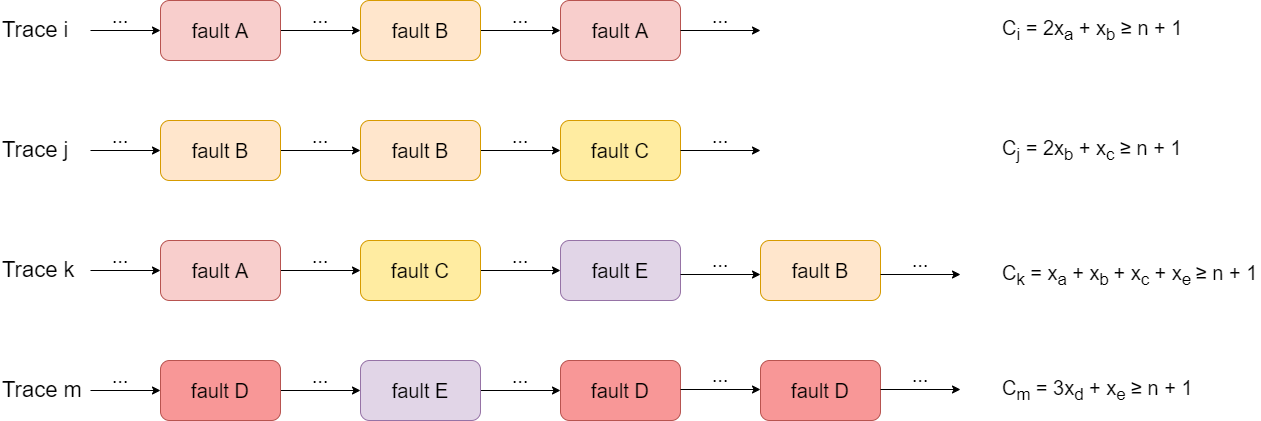
\includegraphics[scale=0.29]{ch5-placement/img/placement-eq.drawio.png}
                    \caption{Inégalités sur les coefficients de protection à partir des attaques}
                    \label{fig:placement-ineq}
                \end{figure}
                
                L'objectif est de trouver les ensembles de coefficients ($\{x_1, ..., x_n\}$) validant les contraintes $C_i$ et minimisant la fonction $x_1 + x_2 + ... + x_n$. 
                Ce problème est une instance du problème d'optimisation linéaire en nombre entier, \gls{ilp}, qui est NP-complet.
        
            \subsubsection{Algorithme de placement réparti optimal}
            \label{sec:placement-optimal-algo}
            
                Le listing \ref{lst:optimal-placement} présente l'algorithme de placement réparti optimal (\textit{rep-opt}) qui s'appuie aussi sur les attaques minimales.
                Dans un premier temps, les contraintes du problème d'optimisation linéaire sont générées à partir des attaques (fonction \texttt{compute\_constraint} ligne 12) et le problème d'optimisation linéaire est résolu dans la fonction \texttt{solve\_ilp} (ligne 14), qui fournit ainsi l'ensemble des coefficients minimisant la somme des protections appliquées.
                Le programme $P'$ est ensuite généré en appliquant les contre-mesures avec les coefficients de protection obtenus.

\lstset{caption={Algorithme de placement réparti optimal \texttt{rep-opt}},label=lst:optimal-placement}
\begin{lstlisting}  
def placement_rep_opt(C: Catalog, P: Program, M: AttackModel, n: int):
    # Get sucessfull non-detected attacks.
    attacks = T_s(P, M, n)
    # Filter with minimals attacks.
    minimals = RedundacyAnalysis(attacks).minimals()
    
    # Initial protection factors Kn at 1 for all IP.
    required_kn = { IPA: 1, IPB: 1, ..., IPN: 1 }
    
    constraints = [] # constraints for ILP
    for attack in minimals:
        constraints += compute_constraint(attack)
    
    required_kn = solve_ilp(constraints, required_kn)
    
    # Generation of P'
    P` = P
    for IP, kn in required_kn:
        S = C.get_cm(IP.model(), kn) # Select protection scheme from catalog
        P` = S(P`, IP) # Apply local protection        
    return P`
\end{lstlisting} 

                Dans le cadre d'un catalogue adapté et complet pour le modèle $m$, $P'$ est robuste en au moins $n$ fautes et la somme des coefficients de protection appliqués est minimale.
    
        \subsection{Autres algorithmes de placement}
        \label{sec:placement-other}

            Trois approches de placement ont été abordées précédemment: le placement systématique (algorithmes \textit{naïf}, \textit{atk} et \textit{min}), le placement par bloc par heuristiques (\textit{bloc-h}) et le placement réparti optimal (\textit{rep-opt}).
            Cette section discute de certaines variantes possibles de ces algorithmes.
            
            \paragraph{Catalogue non total}
            Les sections précédentes ont considéré des catalogues qui possèdent toujours un schéma de protection avec le coefficient de protection demandé.
            On considérera ici un catalogue non total, qui dispose d'une fonction \textit{catalog.get\_cm(IP, k)}, retournant le couple $(S, k')$, avec $S$ le schéma de protection et $k'$ le coefficient de protection de $S$. Deux cas peuvent être distingués : 
            \begin{itemize}
                \item \textit{Sur-protection} : le catalogue fournit le schéma de protection avec $k'$ le plus petit, tel que $k' > k$.
                \item \textit{Sous-protection} : le catalogue fournit un schéma avec $k' < k$.
            \end{itemize}
    
            La \textit{sur-protection} préserve la robustesse du programme protégé. Dans le cas de l'algorithme optimal néanmoins, il devient nécessaire d'ajouter une contrainte supplémentaire sur les coefficients de protection requis pour certains \gls{ip}s. Cela peut donc faire sortir le problème du cadre de l'\gls{ilp} (ce qui ne le rend pas pour autant indécidable), en ajoutant des contraintes du type $X_a \neq 2$ (pour représenter l'absence de schéma pour $K_n = 2$).
            Dans le cas d'une \textit{sous-protection}, le problème de sortie du cadre du problème \gls{ilp} se pose aussi.
            Plus encore, la robustesse du programme peut être remise en question. Si un autre \gls{ip} peut être protégé avec un coefficient de protection suffisant, alors il est possible de garantir la robustesse du programme (quelle que soit l'approche de placement utilisée).
            S'il existe des traces d'attaques pour lesquelles il n'est pas possible de protéger pour $n$ fautes en raison d'un manque de schéma de protection adapté, alors la robustesse en $n$ fautes du programme $P'$ est perdue.
            Ces traces d'attaques sont cependant connues au moment du placement et peuvent être retournées à l'utilisateur, permettant d'anticiper les traces d'attaques du programme $P'$ sans avoir à en explorer les chemins fautés et de déterminer le nombre de fautes pour lequel $P'$ est robuste (en calculant la somme des coefficients de protection des \gls{ip} de chaque attaque non protégée).
             
            \paragraph{Placement réparti par heuristique}
            On peut construire l'algorithme \textit{rep-h} correspondant au placement réparti utilisant des heuristiques plutôt qu'un problème \gls{ilp}.
            Cet algorithme fonctionne comme \textit{bloc-h} (listing \ref{lst:placement-bloc-h}), en combinant une heuristique de parcours des traces et une heuristique de sélection des \gls{ip}s à protéger dans une trace.
            Cette approche peut être préférée à l'approche \textit{rep-opt} (listing \ref{lst:optimal-placement}) dans le cas où :
            \begin{itemize}
                \item le problème \gls{ilp} de l'approche optimale est trop complexe pour être résolu.
                \item certaines contraintes sur le catalogue sortent du cadre du problème \gls{ilp} standard.
            \end{itemize}
             
            \paragraph{Placement optimal par bloc}         
            L'algorithme \textit{bloc-h} ne garantit pas l'optimalité du placement par bloc. Un algorithme de placement optimal par bloc (visant à protéger le moins d'\gls{ip}s possible avec un $K_n = n+1$) est envisageable.
            Le placement \textit{bloc-h} nécessite cependant des contraintes qui ne sont pas de l'ordre du problème \gls{ilp} (les coefficients n'étant plus bornés entre $1$ et $n + 1$ mais ne pouvant prendre que l'une des deux valeurs).
            Cet algorithme correspond à rechercher l'ensemble minimum d'\gls{ip} qui couvrent toutes les traces d'attaques minimales au moins une fois, ce qui se rapproche de l'algorithme de sélection présenté dans le chapitre suivant (voir section \ref{sec:ch6-impl-selection}). 
            
    \section{Expérimentation}
    \label{sec:placement-exps}
        
        Cette section présente quelques expérimentations qui ont été menées sur les algorithmes de placement présentés précédemment : 
        \begin{itemize}
            \item \textit{naïf} (section \ref{sec:placement-syst}) : protection avec $K_n = n+1$ de tous les \gls{ip}s du programme.
            \item \textit{atk} (section \ref{sec:placement-syst}) : protection avec $K_n = n+1$ de tous les \gls{ip}s intervenant dans les attaques.
            \item \textit{min} (section \ref{sec:placement-syst}) : protection avec $K_n = n+1$ de tous les \gls{ip}s intervenant dans les attaques minimales.
            \item \textit{bloc-h} (section \ref{sec:placement-bloc}) : protection avec $K_n = n+1$ d'au moins un \gls{ip} par attaque minimale avec heuristiques.
            \item \textit{rep-opt} (section \ref{sec:placement-opti}) : algorithme optimal pour la protection répartie entre les \gls{ip}s.
        \end{itemize}
            
        \begin{figure}[!h]\centering
            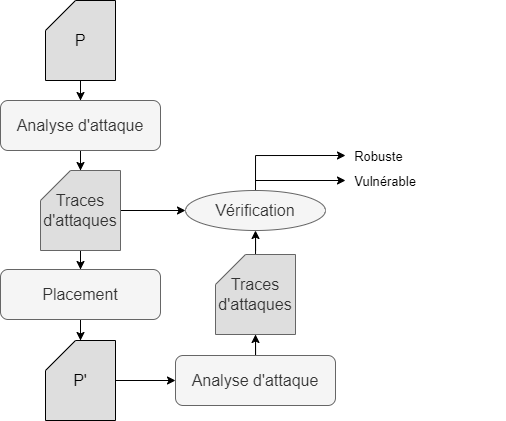
\includegraphics[scale=0.45]{ch5-placement/img/placement-exps.drawio.png}
            \caption{Méthodologie expérimentale pour les algorithmes de placement}
            \label{fig:placement-exp-clpp}
        \end{figure}
        
        La figure \ref{fig:placement-exp-clpp} présente la méthodologie expérimentale utilisée. Chaque algorithme prend en entrée les traces d'attaques générées par Lazart, et retourne les protections à appliquer pour générer le programme $P'$. 
        Une analyse d'attaque est effectuée sur $P'$, permettant ainsi de déterminer si le programme est robuste en $n$ fautes (ce qui n'est garantit que si l'exécution symbolique est complète et correcte).
        Pour l'algorithme de placement optimal (\textit{rep-opt}), la résolution du problème d'optimisation linéaire a été réalisée avec un outil en ligne \footnote{L'annexe \ref{annexe:ilp-memcmp} présente les fichiers de contraintes fournis à l'outil en ligne (\url{https://online-optimizer.appspot.com}).}.
        
        La section \ref{sec:placement-exp-cms} décrit les catalogues de contre-mesures utilisés en fonction du modèle de faute considéré.
        La section \ref{sec:placement-exp-prgm} présente les programmes étudiés et les objectifs d'attaques et la section \ref{sec:placement-exp-res} discute des résultats obtenus.

        \subsection{Catalogue de contre-mesures et inversion de branches}
        \label{sec:placement-exp-cms}

            La section \ref{sec:ch6-defs} a présenté la contre-mesure de multiplication de tests qui est adaptée pour le modèle de l'inversion de test.
            Ses schémas de protection protègent à la fois la branche \textit{vrai} et la branche \textit{faux} de chaque test.

            Dans ces expérimentations, on s'intéressera à une variation de cette contre-mesure qui vise à protéger une seule branche d'un test, permettant ainsi de protéger chaque branche avec une pondération différente.
            Cela nécessite de considérer un autre modèle que l'inversion de test, qu'on appellera \textit{inversion de branche} (\gls{BI}), et pour lequel les points d'injection de la branche \textit{vrai} et la branche \textit{faux} sont distincts.

            Lazart ne supporte pas directement le modèle de l'inversion de branche, mais il est possible d'appliquer une analyse en inversion de test et de distinguer à posteriori les fautes concernant la branche \textit{vrai} et la branche \textit{faux}.

            Les expérimentations utilisent un catalogue de contre-mesures complet et adapté pour le modèle de faute considéré. Ce catalogue retourne le schéma de protection à appliquer pour un point d'injection et un coefficient de protection donnés. 
            Dans le cadre de \gls{BI}, on utilisera donc la multiplication de test sur la branche correspondant au point d'injection.
            Pour le modèle \gls{DL}, on utilisera la multiplication de load.
            Le catalogue garantit ainsi qu'un schéma de protection de profondeur $n$ offre un coefficient de protection de $n + 1$.
        
        \subsection{Programmes utilisés}
        \label{sec:placement-exp-prgm}

            Les programmes étudiés dans cette section sont les suivants:
            \begin{itemize}
                \item \textit{verify pin 2b} (\texttt{vp2b}).
                \item \textit{firmware updater 1} (\texttt{fu1}).
                \item \textit{memcmps} (\texttt{memcmps3}).
            \end{itemize}
    
            \texttt{vp2b} correspond à une version modifiée de \textit{verify\_pin} 2 (voir annexe \ref{annexe:prgm:vp2b}), qui comprend les booléens endurcis et la boucle en temps constant mais ne possède pas de contre-mesure vérifiant le compteur de boucle (l'idée étant de placer les schémas de protection). \texttt{vp2b} est analysé uniquement avec le modèle \gls{BI} et avec l'objectif d'attaque visant à s'authentifier avec un \gls{pin} faux. Les tableaux d'entrées sont symboliques, de taille 4 et différents sur au moins un octet.
    
            \texttt{fu1} (voir section \ref{sec:lz:exp:bench}) à l'inverse contient une duplication de test systématique et considère les modèles \gls{BI} et \gls{DL}. L'objectif d'attaque vise soit à charger un micro-programme corrompu, soit à ne pas mettre à jour le micro-programme.
    
            \texttt{memcmps3} correspond à une version durcie du programme présenté dans la section \ref{sec:lz:memcmps} (voir annexe \ref{annexe:prgm:memcmps3}), dans laquelle quatre appels successifs à \texttt{memcmp} sont effectués avec différents masques. Les tableaux d'entrées sont symboliques et différents (sur au moins un octet) et l'objectif est de retourner $vrai$ malgré l'inégalité des tableaux.
            Le programme est analysé avec les modèles \gls{BI} et \gls{DL}. 
        
        \subsection{Comparaison des algorithmes de placement}
        \label{sec:placement-exp-res}

            La table \ref{tbl:placement-exp-clpp} présente les résultats obtenus pour les différents programmes.
            La colonne "Expé" indique les paramètres de l'expérimentation avec "P" le programme utilisé, "m" le modèle de faute considéré et "IPs" le nombre total de points d'injection dans le programme.
            La colonne "Algos" indique quel algorithme de placement est utilisé.
            La colonne "$\sum$ de protections" indique la somme des pondérations de protection\footnote{Correspondant au coefficient de protection appliqué pour chaque \gls{ip} moins 1 (un \gls{ip} non protégé ayant un coefficient de protection de 1).} appliquées par le placement.
            Enfin la colonne "Robuste" indique si le programme protégé $P'$ est robuste en $n$ fautes après une analyse de vérification avec Lazart.
            
            \begin{table}[htp]
                {\small
                \begin{center}
                    \begin{tabular}{lll|l|llll|l}
                    \multicolumn{3}{c}{Expé} & \multicolumn{1}{c}{Algo.} & \multicolumn{4}{c}{$\sum$ des protections} & \multicolumn{1}{c}{Robuste} \\
                    \hline
                    P & m & IPs &  & 1 faute & 2 fautes & 3 fautes & 4 fautes &  \\
                    \hline
                    \hline
                    \texttt{vp2b} & BI & \multicolumn{1}{r|}{8} & naïf & 8 & 16 & 24 & 32 & \checkmark \\
                     &  &  & atk & \textbf{3} & 8 & 12 & 16 & \checkmark \\
                     &  &  & min & \textbf{3} & 8 & 12 & 16 & \checkmark \\
                     &  &  & bloc-h & \textbf{3} & \textbf{6} & \textbf{9} & \textbf{12} & \checkmark \\
                     &  &  & rep-opt & \textbf{3} & \textbf{6} & \textbf{9} & \textbf{12} & \checkmark \\
                    \hline
                    \hline
                    \texttt{fu1} & BI & \multicolumn{1}{r|}{42} & naïf & 42 & 84 & 126 & 168 & \checkmark \\
                     &  &  & atk & \textbf{0} & 28 & 42 & 88 & \checkmark \\
                     &  &  & min & \textbf{0} & 28 & 42 & 72 & \checkmark \\
                     &  &  & bloc-h & \textbf{0} & 14 & 21 & 28 & \checkmark \\
                     &  &  & rep-opt & \textbf{0} & \textbf{7} & \textbf{14} & \textbf{21} & \checkmark \\
                    \hline
                     & DL & \multicolumn{1}{r|}{2} & naïf & 2 & 4 & 6 & 8 & \checkmark \\
                     &  &  & atk & \textbf{1} & 4 & 6 & 8 & \checkmark \\
                     &  &  & min & \textbf{1} & \textbf{2} & \textbf{3} & \textbf{4} & \checkmark \\
                     &  &  & bloc-h & \textbf{1} & \textbf{2} & \textbf{3} & \textbf{4} & \checkmark \\
                     &  &  & rep-opt & \textbf{1} & \textbf{2} & \textbf{3} & \textbf{4} & \checkmark \\
                    \hline
                     & BI+DL & \multicolumn{1}{r|}{44} & naïf & 44 & 88 & 132 & 176 & \checkmark \\
                     &  &  & atk & \textbf{1} & 32 & 60 & 96 & \checkmark \\
                     &  &  & min & \textbf{1} & 32 & 60 & 80 & \checkmark \\
                     &  &  & bloc-h & \textbf{1} & 16 & 24 & 32 & \checkmark \\
                     &  &  & rep-opt & \textbf{1} & \textbf{9} & \textbf{17} & \textbf{25} & \checkmark \\
                    \hline
                    \hline
                    \texttt{memcmps3} & BI & \multicolumn{1}{r|}{12} & naïf & 12 & 24 & 36 & 48 & \checkmark \\
                     &  &  & atk & \textbf{0} & \textbf{0} & \textbf{0} & 16 & \checkmark \\
                     &  &  & min & \textbf{0} & \textbf{0} & \textbf{0} & 16 & \checkmark \\
                     &  &  & bloc-h & \textbf{0} & \textbf{0} & \textbf{0} & 4 & \checkmark \\
                     &  &  & rep-opt & \textbf{0} & \textbf{0} & \textbf{0} & \textbf{1} & \checkmark \\
                    \hline
                     & DL & \multicolumn{1}{r|}{15} & naïf & 15 & 30 & 45 & 60 & \checkmark \\
                     &  &  & atk & \textbf{1} & 6 & 15 & 32 & \checkmark \\
                     &  &  & min & \textbf{1} & 6 & 15 & 32 & \checkmark \\
                     &  &  & bloc-h & \textbf{1} & 4 & 6 & 8 & \checkmark \\
                     &  &  & rep-opt & \textbf{1} & \textbf{3} & \textbf{4} & \textbf{7} & \checkmark \\
                    \hline
                     & BI+DL & \multicolumn{1}{r|}{27} & naïf & 27 & 54 & 81 & 108 & \checkmark \\
                     &  &  & atk & \textbf{1} & 8 & 24 & 56 & \checkmark \\
                     &  &  & min & \textbf{1} & 8 & 24 & 56 & \checkmark \\
                     &  &  & bloc-h & \textbf{1} & 6 & 9 & 12 & \checkmark \\
                     &  &  & rep-opt & \textbf{1} & \textbf{3} & \textbf{4} & \textbf{9} & \checkmark
                    \end{tabular}
                \end{center}
                }
                \label{tbl:placement-exp-clpp}
                \caption{Comparaison des différents algorithmes de placement}
            \end{table}

            Comme attendu, l'approche par bloc (\textit{bloc-h}) offre de meilleurs résultats que les approches systématiques. De la même manière, le placement réparti (\textit{rep-opt}) produit un poids de protection plus faible.
            
            Pour l'exemple \texttt{vp2b}, on constate que les algorithmes \textit{min} et \textit{atk} sont équivalents, tous les \gls{ip}s des attaques intervenant aussi dans les attaques minimales.
            Les algorithmes \textit{bloc-h} et \textit{rep-opt} fournissent les mêmes résultats, ce qui s'explique par un grand nombre d'attaques en 1 faute qui imposent une pondération de $n \in \mathbb{N}^*$ aux points d'injection concernés pour être résistant en $n$ fautes.

            Pour \texttt{fu1}, seuls deux points d'injection sur les données sont présents et l'un d'entre eux intervient dans une attaque en une faute. Ce même point d'injection est donc à protéger avec un coefficient de protection $K_n = n + 1$ dans le cas du modèle $BI + DL$.
            On observe pour le modèle $BI + DL$ que les algorithmes proposent tous des résultats différents, mettant en évidence la relation d'ordre entre les résultats de chaque algorithme. 

            Pour l'exemple \texttt{memcmps3}, on peut constater un net avantage des algorithmes prenant en compte les attaques pour le modèle \gls{BI}. En effet, une seule attaque est possible avec ce modèle, et consiste à inverser chacun des quatre appels à \texttt{memcmp}. 
            L'algorithme optimal ne nécessite qu'un coefficient de protection $K_n = 2$ puisque déjà quatre fautes sont nécessaires pour l'attaque. 
            Dans cet exemple, les résultats pour l'algorithme \textit{rep-opt} sont meilleurs que \textit{bloc-h} quel que soit le modèle de faute.
            
            On peut remarquer que le programme $P'$ est robuste pour toutes les expérimentations réalisées. Cela peut faire penser que l'exploration des chemins est complète pour tous les programmes.
            Cependant, on peut postuler que si l'exploration rate des chemins pour la génération des attaques sur $P$, il est probable que les chemins correspondant dans $P'$ sont eux aussi manqués.

    \section{Protégeabilité et contre-mesure parfaite}
    \label{sec:model-protectability}

        Les différents algorithmes de placement présentés dans ce chapitre posent des conditions fortes sur les propriétés des contre-mesures du catalogue (adéquation et coefficient de protection suffisant) lorsqu'on recherche une robustesse en $n$ fautes.
        Cette section propose une classification des modèles de faute en fonction du type de protection qu'il est possible d'y appliquer.
        
        On notera $\mathcal{M}$ l'ensemble des modèles de faute.
        Il existe des modèles pour lesquels il est possible de protéger un programme pour le rendre résistant en $n$ fautes, on dit alors que le modèle de faute est \textit{protégeable} (comme les modèles \gls{TI} et \gls{DL}).
        A l'inverse, il existe des modèles pour lesquels il n'est pas possible de se protéger en $n$ fautes. Given et al \cite{Given/ICESS17} ont montré l'existence de tels modèles en se ramenant à des machines de Turing.
        C'est le cas par exemple d'un modèle de remplacement d'instruction arbitraire, permettant de remplacer le programme en un autre de taille arbitraire.
        On divisera donc l'ensemble des modèles de faute en fonction de leur \textit{protégeabilité}:
        
        \begin{itemize}
            \item $\mathcal{P}$ (\textit{modèles Protégeables}): $m \in \mathcal{P} \iff  \exists C $ tel que $\forall \; programme \; P, \forall n \in \mathbb{N}$, $T_s(C(P), m_n) = \emptyset$\footnote{Avec $T_s(P, m_n)$ correspondant à l'ensemble des attaques réussies pour $P$ jusqu'à $n$ fautes.}.
            \item $\mathcal{N}$ (\textit{modèles Non protégeables}): $m \in \mathcal{P} \iff  \nexists C $ tel que $\forall \; programme \; P, \forall n \in \mathbb{N}$, $T_s(C(P), m_n) = \emptyset$ 
        \end{itemize}
        
        L'ensemble des modèles protégeables $\mathcal{P}$ peut être divisé en deux sous-ensembles.
        Les modèles pour lesquels il existe une Contre-mesure Locale Pondérée et Adaptée (CLP-A) sont dits \textit{localement protégeables}, notés  $\mathcal{L}$ et ceux pour lesquels il n'en existe pas sont appelés \textit{globalement protégeables}, notés $\mathcal{G}$. 
        Les modèles pour lesquels il existe une contre-mesure locale parfaite sont dits \textit{parfaitement protégeables}, notés $\mathcal{F}$.
        
        Dans le cas des modèles non protégeables ($\mathcal{N})$, on peut là encore diviser entre ceux pour lesquels il est possible de rendre les attaques plus difficiles à réaliser, qu'on appellera \textit{modèles diluables} $\mathcal{D}$ et ceux pour lesquels cela n'est pas possible, appelés \textit{modèles strictement non protégeables}, notés $\mathcal{S}$.
        
        \begin{figure}[!h]\centering
            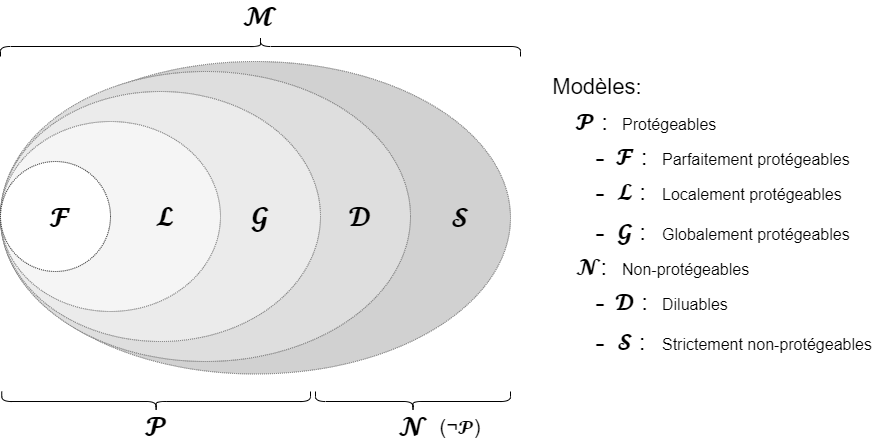
\includegraphics[scale=0.4]{ch5-placement/img/protectable-models-set-extended.drawio.png}
            \caption{Classification des modèles d'attaquant en fonction de leur \textit{protegeabilité}}
            \label{fig:models-protectability}
        \end{figure}
        
        La figure \ref{fig:models-protectability} présente une classification des modèles d'attaquant en fonction de leur protégeabilité. 
        Plusieurs questions restent en suspens concernant l'existence de certaines sous-classes.
        Les sections précédentes ont présenté des modèles dans $\mathcal{L}$ (\textit{localement protégeables}), avec les exemples des modèles \gls{TI}, \gls{DL} et $TI+DL$, pour lesquelles les contre-mesures locales \gls{TM}, \gls{LM} et \gls{TLM} ont été proposées.
        Les modèles \textit{globalement protégeables} ($\mathcal{G}$) sont des modèles pour lesquels il existe une transformation du programme (non locale) permettant de rendre le programme robuste en $n$ fautes. L'existence de cette classe de modèles est hypothétique puisque nous n'avons pas trouvé d'exemple, mais ne semble pas impossible pour autant.
        Il semble difficile de construire une contre-mesure parfaite pour les modèles \gls{TI} et \gls{DL} par exemple, mais l'existence de modèles dans $\mathcal{F}$ semble tout de même probable, si l'on s'intéresse à des modèles de faute simples.
        Formulé autrement: $\mathcal{L} = \mathcal{G} = \mathcal{P} ?$ (considérant que $\mathcal{G}$ n'inclut pas $\mathcal{L})$.
        
        Une autre question survient avec cette classification: est-ce qu'un modèle peut changer de classe de \textit{protégeabilité} si on s'intéresse qu'à un sous-ensemble des programmes possibles à protéger et/ou à un sous-ensemble des objectifs d'attaque.
        Il est aussi possible que cette classification n'ait de sens que si on exclut effectivement certains programmes et objectifs d'attaque qui sont toujours \textit{protégeables} ou \textit{non protégeables} quel que soit le modèle de faute \footnote{Par exemple si un modèle $m$ est non protégeable dans le cas général, mais protégeable si on exclut le programme vide, peut-être faudrait-il le considérer comme protégeable et simplement exclure ce cas extrême de la définition.}.
        Cette question n'a pas été explorée davantage.    
        On peut aussi noter que ce n'est pas parce qu'un modèle de faute est non protégeable qu'il n'existe pas de protection contre ce type d'attaques en considérant un autre niveau de représentation.
        
        Enfin, il est raisonnable de se demander à quel point les modèles \textit{localement protégeables} ($\mathcal{L})$ sont suffisamment réalistes pour être utilisés pour le placement de contre-mesures en pratique.
        On peut arguer à cette question que, même s'il s'avère que les modèles dans $\mathcal{L}$ sont en réalité trop rares ou trop spécifiques, il reste envisageable que cette méthodologie puisse être généralisée pour le calcul du placement de contre-mesures pour des modèles dans $\mathcal{G}$.
        
        Cette classification des modèles en fonction de leur protégeabilité contient donc encore des classes qui sont hypothétiques et des travaux futurs pourraient viser à préciser cela.
    
    \section{Conclusion et perspectives}
    \label{sec:placement-fw}
    
        Cette section présente une conclusion de ce chapitre et discute des perspectives possibles de ces travaux.
        
        \subsection{Conclusion}
        
            La table \ref{tbl:placement-conclusion} présente une comparaison des algorithmes de placement présentés dans ce chapitre (identifiés en colonne "Algo"):
            \begin{itemize}
                \item \textit{naïf}: protection systématique de tous les \gls{ip}s avec $K_n = n + 1$.
                \item \textit{atk}: protection des \gls{ip}s des attaques avec $K_n = n + 1$.
                \item \textit{min}: protection des \gls{ip} des attaques minimales avec $K_n = n + 1$.
                \item \textit{bloc-h}: algorithme par bloc avec heuristiques.
                \item \textit{rep-opt}: algorithme optimal réparti.
                \item \textit{bloc-opt}: algorithme par bloc optimal.
                \item \textit{rep-h}: algorithme réparti avec heuristiques.
            \end{itemize}
            La colonne "Type" indique le type de placement de l'algorithme: \textit{systématique}, par \textit{bloc} ou \textit{réparti}.
            Les colonnes "Garanties $P'$" indiquent les garanties pour le programme $P'$ en ce qui concerne la robustesse du programme $P'$ pour un catalogue total. L'optimalité du placement indique si le placement est optimal par rapport au type de placement considéré.            
            La colonne "Complexité" indique la complexité de l'algorithme de placement (donc sans prendre en compte les différentes analyses d'attaques, de points chauds ou de redondance éventuelles), $t$ correspondant au nombre d'attaques minimales obtenues par l'analyse d'attaque.
            Les colonnes "Analyses" indiquent les analyses de Lazart utilisées pour l'algorithme: analyse d'attaques ($AA$), analyse de redondance ($Red$) et analyse de points chauds ($HS$).

            \begin{table}[h]
                {\small
                \begin{center}
                    \begin{tabular}{l|l|ll|l|lll}
                    Algorithme & Type & \multicolumn{2}{l|}{Garanties $P'$} & Complexité & \multicolumn{3}{l}{Analyses requises} \\
                     &  & Robuste & Optimal &  & AA & Red & HS \\
                     \hline
                    naïf & syst. & \checkmark & - & $O(t)$ & \checkmark & - & - \\
                    atk & syst. & \checkmark & - & $O(t)$ & \checkmark & - & - \\
                    min & syst. & \checkmark & - & $O(t)$ & \checkmark & \checkmark & - \\
                    bloc-h & bloc & \checkmark & - & $O(t)$ & \checkmark & \checkmark & \checkmark \\
                    rep-opt & réparti & \checkmark & \checkmark & NP-Complet$^1$ & \checkmark & \checkmark & - \\
                    bloc-opt & bloc & \checkmark & \checkmark & NP-Complet$^1$ & \checkmark & \checkmark & - \\
                    rep-h & réparti & \checkmark & - & $O(t)$ & \checkmark & \checkmark & \checkmark
                    \end{tabular}
                \end{center} 
                }
                
                \caption{Comparaison des différentes approches de placement}
                \label{tbl:placement-conclusion}
            \end{table}
            
            \footnotetext[1]{L'\gls{ilp} est NP-Complet dans le cas général mais les contraintes générées dans le cas des placements optimaux restent relativement simples.}
  
            Les expérimentations ont montré que les différents algorithmes parviennent à rendre un programme robuste en $n$ fautes lorsque le catalogue est total. 
            On peut constater la relation d'ordre attendue entre les poids de protections proposés par les différents algorithmes de placement : \textit{naïf} $\geq$ \textit{atk} $\geq$ \textit{min} $\geq$ \textit{bloc-h} $\geq$ \textit{bloc-opt} $\geq$ \textit{rep-h} $\geq$ \textit{rep-opt}. 
            Les algorithmes de placement systématiques produisent un grand nombre de protections superflues par rapport aux autres approches, mais les résultats dépendent grandement du programme considéré, \textit{min} trouvant le placement optimal dans l'exemple \texttt{fu1} avec \gls{DL} par exemple.
            De la même manière, \textit{bloc-h} peut parfois donner les mêmes résultats que \textit{rep-opt}, comme pour \texttt{vp2b}.
            
            La complexité du placement optimal (section \ref{sec:placement-opti}) rend son passage à l'échelle difficile pour des programmes contenant des combinaisons de placements possibles élevées. Néanmoins, les expérimentations tendent à montrer que l'ensemble des contraintes générées pour le problème d'optimisation linéaire est souvent simple, même dans le cas de programmes complexes. Cela est du aux attaques en une faute imposant un coefficient de protection maximal (c'est-à-dire de $n + 1$) à certains points d'injection.
            
            L'analyse en isolation (section \ref{sec:ooc}) des schémas de protection permet d'obtenir des garanties en fautes multiples concernant l'efficacité d'une contre-mesure sur un point d'injection, en fonction d'un modèle de faute. En combinaison avec l'exploration des chemins fautés, il est possible d'anticiper les comportements des programmes protégés en fonction des coefficients de protection appliqués.
            Dans le cas de catalogue non totaux, il est possible de prévoir si un placement va produire un programme $P'$ robuste si un cas de sous-protection est rencontré (section \ref{sec:placement-other}), et dans ce cas de fournir les attaques de $P'$.
            Si l'exploration des chemins d'attaque n'est pas complète, on a tout de même la garantie d'avoir protégé certaines attaques sans en avoir introduit de nouvelles, ce qui permet à $P'$ d'être \textit{au moins aussi robuste} que $P$, sans garantie de robustesse en $n$ fautes.
    
        \subsection{Perspectives}
        
            Différentes perspectives peuvent être envisagées pour les travaux présentés dans ce chapitre. Dans un premier temps, il serait intéressant d'étendre les exemples de programmes et de contre-mesures pour comparer plus en profondeur les diverses approches.
            Les algorithmes \textit{bloc-opt} et \textit{rep-h} pourraient être implémentés afin de pouvoir les comparer expérimentalement avec les autres algorithmes, mais ils n'offriront pas de meilleures garanties que \textit{rep-opt}.            
            Pour terminer sur le plan implémentation, l'algorithme de placement optimal utilise pour le moment une intervention manuelle de l'utilisateur pour l'appel à un outil d'optimisation linéaire et automatiser ce processus serait un plus.
            
            De la même manière, d'autres modèles de faute pourraient être considérés, notamment avec des modèles tels que le saut inconditionnel impliquant plusieurs points d'entrée et de sortie dans le schéma de protection, dans le cas de l'analyse de contre-mesures en isolation.
            Substituer les \gls{ip}s protégés aux \gls{ip}s non protégés dans l'exploration des chemins fautés nécessiterait de couvrir les comportements possibles de ces différents points d'entrée ou de sortie.

            \begin{sloppypar}
            L'analyse en isolation de contre-mesures propageant des états internes \cite{Oh/TR02, lalande} nécessite de prendre en compte ces états comme entrées et sorties du schéma de protection.
            Cela nécessiterait potentiellement de diviser les scénarios de l'analyse en isolation en séparant les entrées liées au point d'injection (comme la condition du branchement) et les entrées correspondants aux états internes.
            \end{sloppypar}
            
            Les algorithmes de placement pourraient être étendus à des contre-mesures à granularité plus hautes que le point d'injection.
            Il s'agirait par exemple de sélectionner une protection au niveau d'un bloc ou d'une fonction plutôt qu'une protection de plusieurs points d'injection. Cependant il est difficile de déterminer dans quel cas chaque protection devrait être utilisée. Une analyse en isolation mais appliquée sur des structures plus grosses qu'un point d'injection pourrait aider à la définition de tels algorithmes.

            Le placement de contre-mesures non locales fait aussi partie des pistes d'exploration.
            Cela implique que l'ordre dans lequel les protections sont appliquées est important pour le placement, les applications n'étant pas indépendantes.
            Il est possible de construire un algorithme de placement basé sur les mêmes heuristiques que \textit{bloc-h}, en sélectionnant une contre-mesure adaptée pour protéger les points d'injection pour chaque attaque.
            Les garanties de robustesse sur un tel placement sont difficiles à définir, les protections ajoutées étant modifiées par l'application des contre-mesures suivantes.
            Une solution pourrait consister à étudier en isolation des schémas de protection combinés des différents schémas de protection du catalogue. 
            
            La classification théorique des modèles de faute en fonction de leur protégeabilité laisse encore quelques points en suspens, notamment en ce qui concerne l'existence de certaines classes de contre-mesures. Prouver l'existence ou la non-existence de ces groupes pourrait permettre d'aider à la définition de schémas de protection.
            
            Les algorithmes de placement présentés dans ce chapitre se basent tous sur une analyse des chemins d'attaques non détectées validant l'objectif d'attaque, et visent à sélectionner les portions du programme à protéger.
            Le chapitre suivant s'intéresse à une approche inverse, visant à déterminer quelles portions de contre-mesures peuvent être retirées dans un programme protégé, en se basant sur une analyse recherchant les chemins d'attaques détectés.